\chapter{Validation}
\label{ch:realdata}

\section{Introduction}

\newthought{Real data tends to carry more surprises} than even the most sophisticated simulation software can reveal.  While the simulation framework we presented in Chapter \ref{ch:simulation} was useful to establish the basic operations and performance of the graphical variant calling algorithm presented in Chapter \ref{ch:methods}, true validation data is useful in establishing filters, traversal parameters, and other parameters for treating real data.  In this chapter, we discuss validation data obtained for this purpose and the insights gleaned by comparing an initial set of calls to this dataset.

\subsection{Data processing for validation isolates}

We focused our validation efforts on the 803xGB4 cross, solely because samples were already in culture, reducing turnaround time from a full year to a few months.  We selected four samples for long-read sequencing on the PacBio RS II instrument.  As of this writing, only two samples have been completed: PG0051-C (the 3D7 clone, useful for verifying assembly quality by comparison with the finished 3D7 reference), and PG0446-C (one of the 803xGB4 progeny); it is currently not certain if and when the other two samples will be reattempted.  The PG0051-C isolate was provided by Susana Campino of the Kwiatkowski lab at the Wellcome Trust Sanger Institute.  The PG0446-C isolate was provided by Michael Krause and Rick Fairhurst at the Malaria Pathogenesis and Human Immunity Unit at the National Institute of Allergy and Infectious Disease.  In both cases, approximately $15~{\mu}g$ of high molecular weight gDNA for each isolate was vacuum-sealed and shipped to the CSHL Pacific Biosciences Sequencing Service\footnote{\url{http://cshl.edu/Research/PacBio.html}}.  Sequencing libraries with an average fragment size of $20$ kb were constructed for each sample and size-selected to remove fragments smaller than $7$ kb and larger than $20$ kb using BluePippin.  Optimal loading concentration was determined by choosing a wide range for each of the first $4$ SMRT cells and selecting the concentration that yielded the highest read yield for the remaining SMRT cells.  The PG0051-C isolate was sequenced in late 2014 with the P5-C3 chemistry and assembled with PacBio's HGAP $2.0$ software (assuming a genome size of $23$ megabases).  The PG0446-C isolate, run $16$ months later, was sequenced with the newer P6-C4 chemistry and HGAP $3.0$ software with the same genome size parameter.  Table \ref{tbl:asmstatspacbio} summarizes the sequencing and assembly results on these two isolates.

\begin{table}[]
\centering
\caption{Assembly statistics for PacBio RS II data on PG0051-C and PG0443-C isolates}
\label{tbl:asmstatspacbio}
\begin{tabular}{@{}lll@{}}
\toprule
                        & PG0051-C (3D7)   & PG0443-C (36F11)   \\ \midrule
Chemistry               & P5-C3            & P6-C4              \\
SMRT cells              & $8$              & $9$                \\
Number of reads         & $245,661$        & $282,459$          \\
N50 read length         & $12,968$ bp      & $14,339$ bp        \\
Assembler               & HGAP $2.0$       & HGAP $3.0$         \\
Average contig coverage & $78$x            & $94$x              \\
Polished contigs        & $34$             & $33$               \\ \bottomrule
\end{tabular}
\end{table}

\subsubsection{Establishing assembly quality}
We examined genome recovery and access to massively repetitive sequence (subtelomeric and centromeric regions) that tend to be inaccessible with Illumina sequencing.  PacBio reads were aligned to the finished 3D7 genome using PacBio's \texttt{blasr} long read alignment tool\footnote{\url{https://github.com/PacificBiosciences/blasr}}, while Illumina reads were mapped with the \texttt{bwa mem} tool.  Two such regions in the Illumina and PacBio data for the PG0051-C isolate are shown in Figure \ref{fig:pacbioregions}.  It is evident that the PacBio coverage is roughly uniform across the entire length of the chromosome. In contrast, the Illumina coverage spikes and dips as it moves along, reaching zero coverage in many regions (especially the biologically interesting subtelomeric repetitive regions).

\begin{figure}[h!]
  \centering
    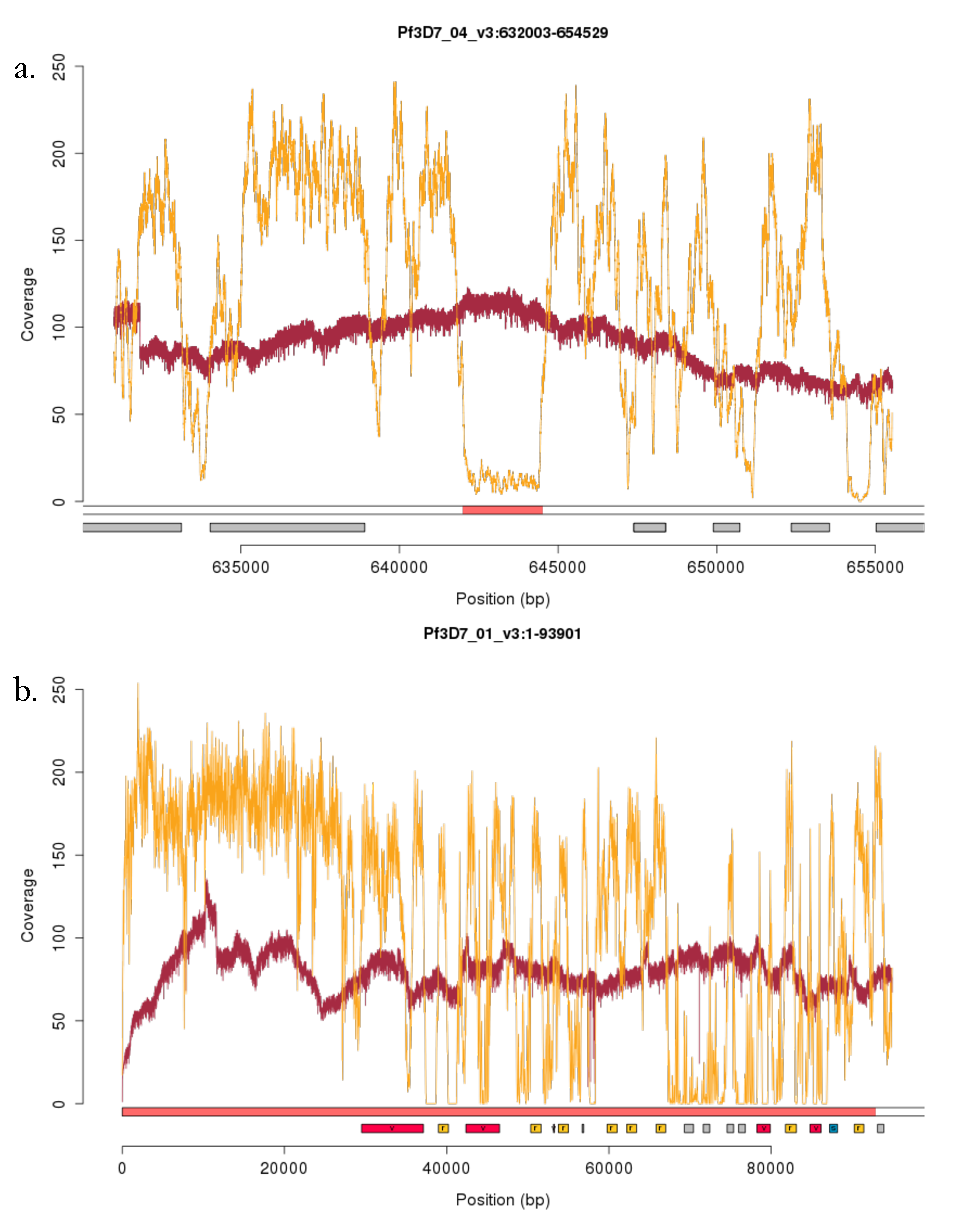
\includegraphics[width=\textwidth]{pacbioregions}
  \caption{Coverage for Illumina data (orange) and PacBio data (red) of the same sample: PG0051-C (the reference isolate, 3D7).  a. Coverage over the chromosome $4$ centromere.  b. Coverage over the $5'$ telomere of chromosome $1$.  Genes from the \textit{var}, \textit{rifin}, and \textit{stevor} antigenic gene families are highlighted as red, orange, and blue rectangles, respectively.}
  \label{fig:pacbioregions}
\end{figure}

We compared the PacBio-produced assembly of the PG0051-C isolate to the finished reference sequence by performing an all-by-all (contigs versus chromosomes) alignment with MUMmer\cite{Versatileandopens:2004dy}.  The alignments are visualized as a multi-dotplot in Figure \ref{fig:dotplot3D7}, an extension of a dot plot that depicts alignments as two dimensional matricies with target and query sequences on the $x$ and $y$ axes, aligning regions of the two sequences shaded accordingly\cite{Gibbs:1970jf}.  Most chromosomes are assembled completely, and the overwhelming majority of the assembly appears on-diagonal (indicating successful one-to-one reconstruction).  Elements appearing off-diagonal could represent misassembly.  However, note that most of these off-diagonal elements occur towards the extremes of each chromosome.  Given that the reference genome was constructed with Sanger reads substantially shorter than the PacBio reads, it is possible some repetitive regions have been collapsed or misplaced, contributing to this nominal error rate.

\begin{figure}[h!]
  \centering
    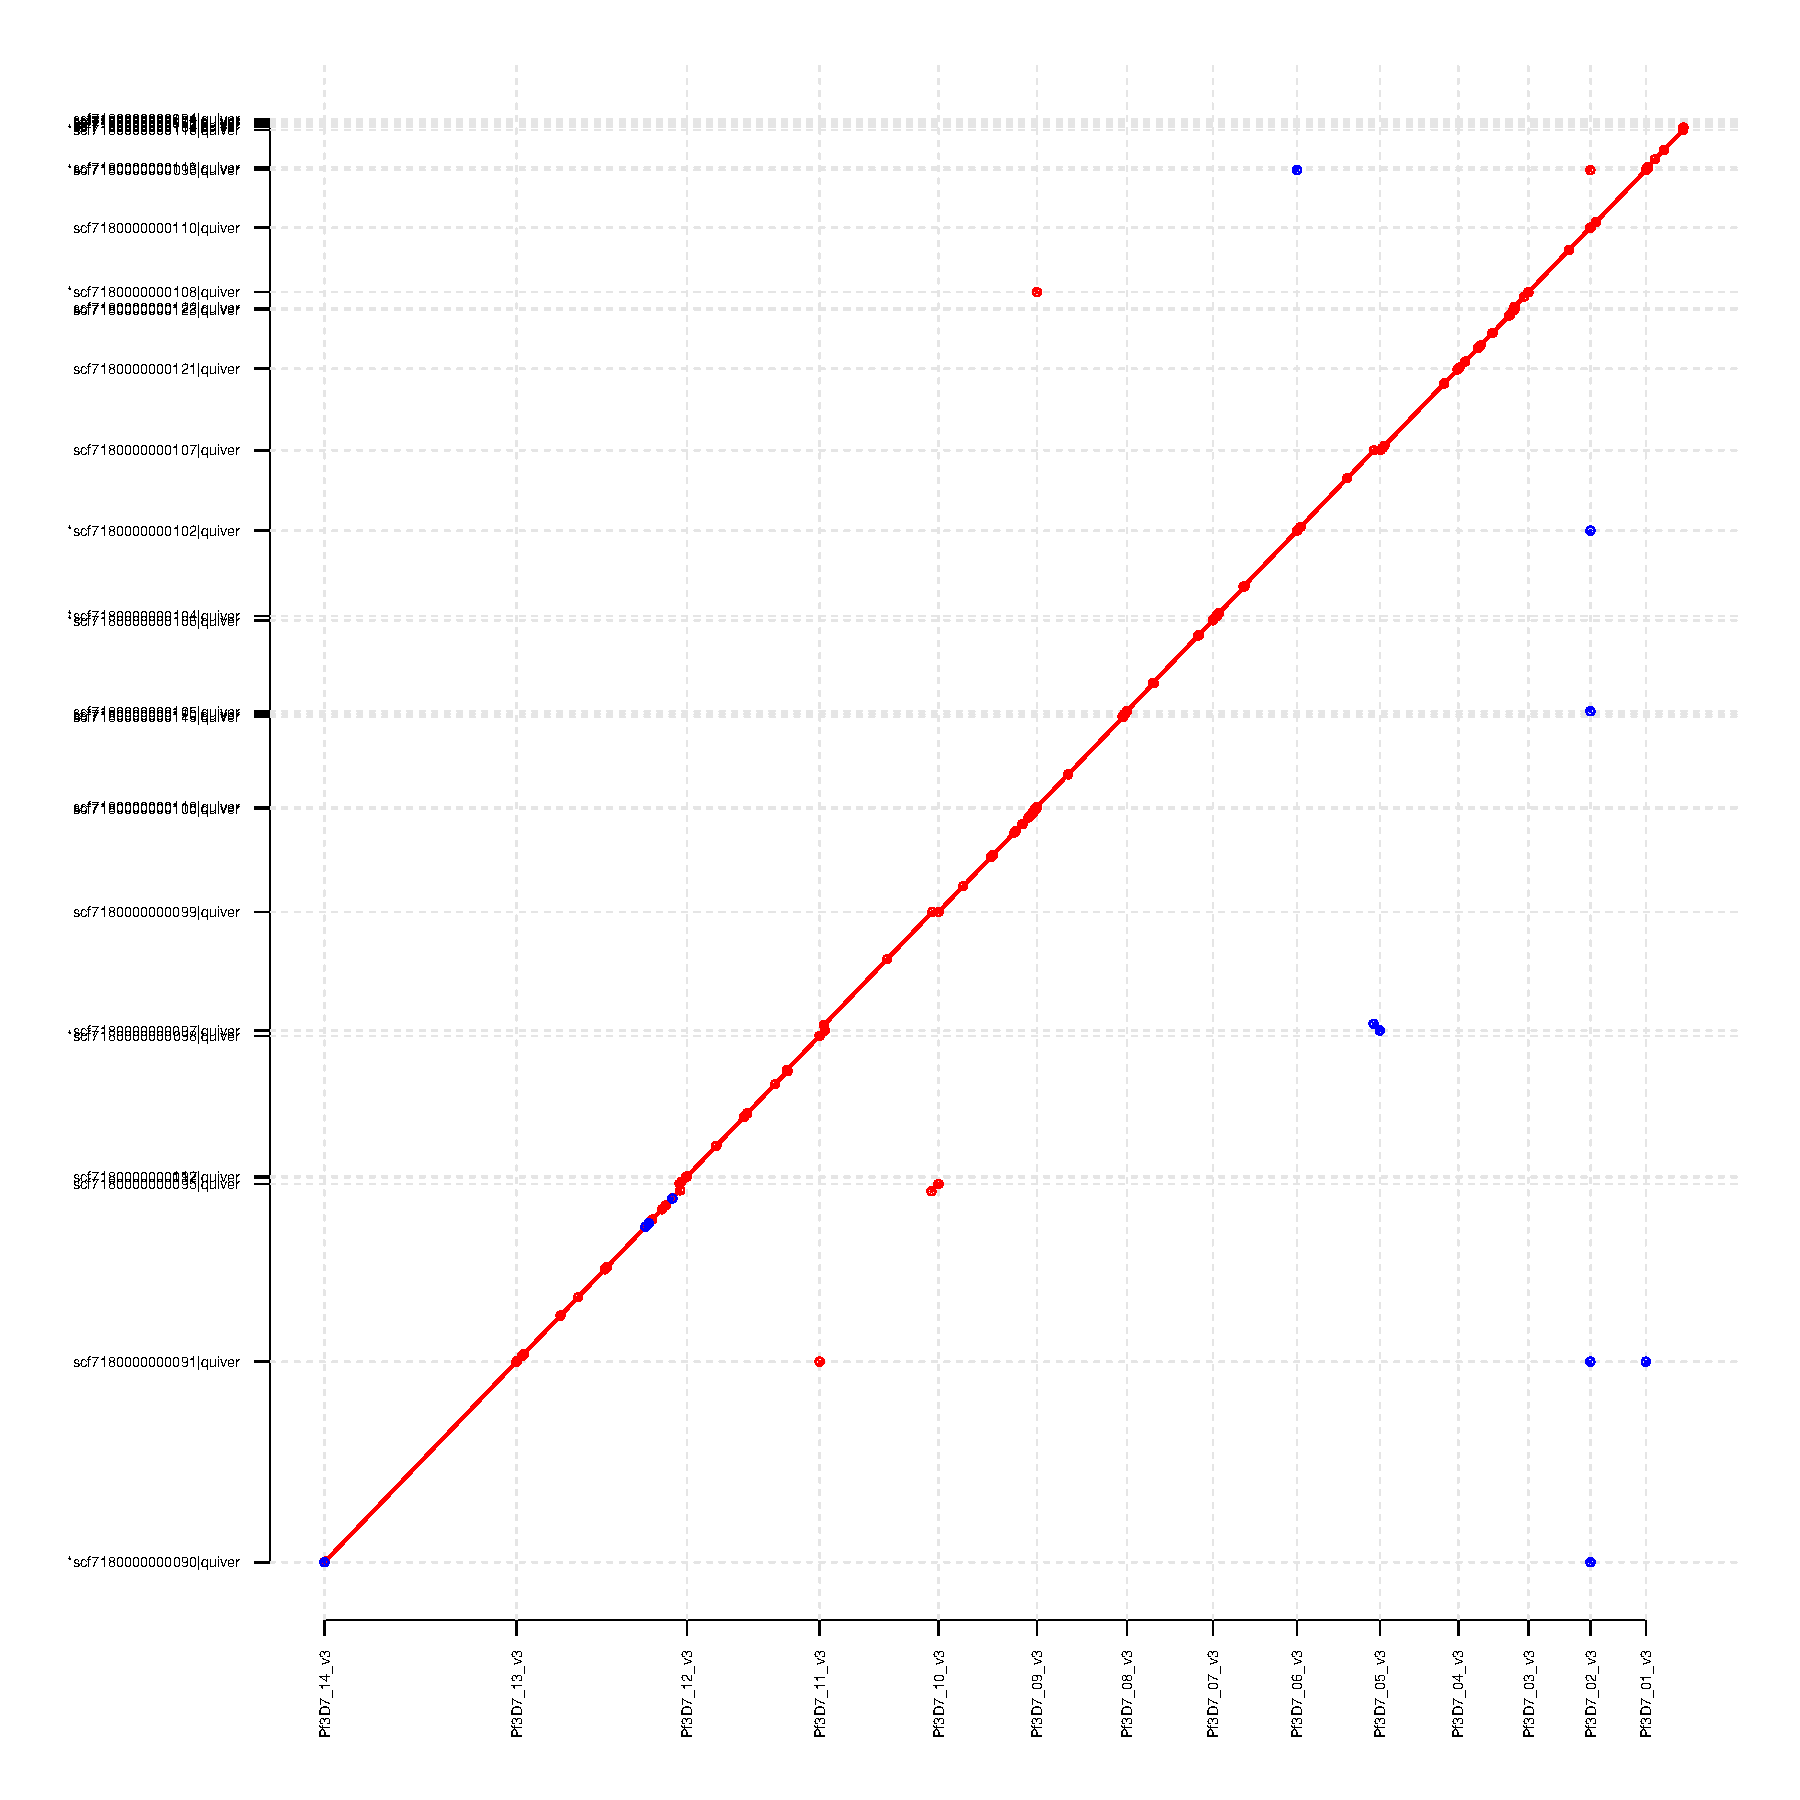
\includegraphics[width=0.7\textwidth]{dotplot}
  \caption{Alignment of contigs from PG0051-C to 3D7 reference assembly, with sequences from reference and draft assembly on the x and y-axis, respectively.  Each contig from the draft assembly is represented by a line segment terminated at either end with circles.  Red denotes forward alignment of contigs to the reference, blue denotes reverse alignment.}
  \label{fig:dotplot3D7}
\end{figure}

\begin{table}[]
\centering
\caption{Apparent errors per chromosome in the PG0051-C assembly}
\label{tbl:asmerrors}
\begin{tabular}{@{}llll@{}}
\toprule
              & SNP              & INS               & DEL              \\
\midrule
Pf3D7\_01\_v3 & $119~(0.02\%)$   & $763~(0.12\%)$    & $291~(0.05\%)$   \\
Pf3D7\_02\_v3 & $164~(0.02\%)$   & $475~(0.05\%)$    & $162~(0.02\%)$   \\
Pf3D7\_03\_v3 & $272~(0.03\%)$   & $523~(0.05\%)$    & $290~(0.03\%)$   \\
Pf3D7\_04\_v3 & $141~(0.01\%)$   & $856~(0.07\%)$    & $713~(0.06\%)$   \\
Pf3D7\_05\_v3 & $111~(0.01\%)$   & $531~(0.04\%)$    & $175~(0.01\%)$   \\
Pf3D7\_06\_v3 & $504~(0.04\%)$   & $731~(0.05\%)$    & $180~(0.01\%)$   \\
Pf3D7\_07\_v3 & $194~(0.01\%)$   & $609~(0.04\%)$    & $320~(0.02\%)$   \\
Pf3D7\_08\_v3 & $134~(0.01\%)$   & $597~(0.04\%)$    & $251~(0.02\%)$   \\
Pf3D7\_09\_v3 & $61~(0.00\%)$    & $713~(0.05\%)$    & $259~(0.02\%)$   \\
Pf3D7\_10\_v3 & $732~(0.04\%)$   & $810~(0.05\%)$    & $308~(0.02\%)$   \\
Pf3D7\_11\_v3 & $310~(0.02\%)$   & $1,008~(0.05\%)$  & $459~(0.02\%)$   \\
Pf3D7\_12\_v3 & $232~(0.01\%)$   & $1,202~(0.05\%)$  & $390~(0.02\%)$   \\
Pf3D7\_13\_v3 & $231~(0.01\%)$   & $1,493~(0.05\%)$  & $409~(0.01\%)$   \\
Pf3D7\_14\_v3 & $152~(0.00\%)$   & $1,309~(0.04\%)$  & $396~(0.01\%)$   \\
Total         & $3,357~(0.03\%)$ & $11,620~(0.10\%)$ & $4,603~(0.04\%)$ \\
\bottomrule
\end{tabular}
\end{table}

As we have sequenced DNA from the 3D7 parasite, any differences should likely reflect errors in the sequence. We therefore called SNPs between the two assemblies to find these errors. The sums are presented in Table \ref{tbl:asmerrors}, as well as the percent of bases per chromosome these errors represent.  Overall, the SNP, insertion, and deletion rates are exceedingly low: amounting to 19,580 events in a 23 megabase genome (0.17\%). The insertion rate is much higher than that of deletions and SNPs, perhaps due to the dominant insertion error mode of the PacBio sequencing instrument. All chromosomes appear reasonably similar in performance.

We examined the recovery of the $62$ members of the \textit{var} gene family by aligning their full-length genomic sequences (exons and introns) to the PG0051-C assembly using \texttt{bwa mem}. All $62$ \textit{var} genes were successfully aligned to the assembly (all had mapping quality greater than $0$; only $1$ had mapping quality less than 60).  $21$ were found to map with $100\%$ identity. The remaining have, on average, $2.46$ mismatches, $1.39$ insertions, and $0.63$ deletions. The overwhelming majority of indels are a single nucleotide in length.

It seemed likely that many of these errors occur in intronic regions where high repetitive sequence content might contribute to misassembly. We investigated this hypothesis by aligning the exons of the \textit{var} genes separately and enumerating errors observed in exons and introns. We ignored $11$ genes with poor exon alignments (i.e. with mapping quality less than $10$). $91.78\%$ of the errors are found in intronic regions. In all cases, exon $2$ of the \textit{var} gene (the short exon) is base-for-base perfect when compared to the canonical reference.

Based on these measurements of the error rate, we estimate the quality of the PacBio assembly of the PG0051-C (3D7) isolate to be approximately $Q31$\footnote{$Q = -10{\log}_{10}(q) = -10{\log}_{10}((11,620 + 4,603 + 3,357)/23,332,831)$}, or less than one error per thousand bases.  We note that this is a pessimistic estimate, based on the assumption that any differences between this and the reference assembly indicate errors in our assembly.  In long, repetitive regions of the genome, this assumption may not be accurate.

\subsubsection{Preparing the validation isolate reference}

\begin{figure}[h!]
  \centering
    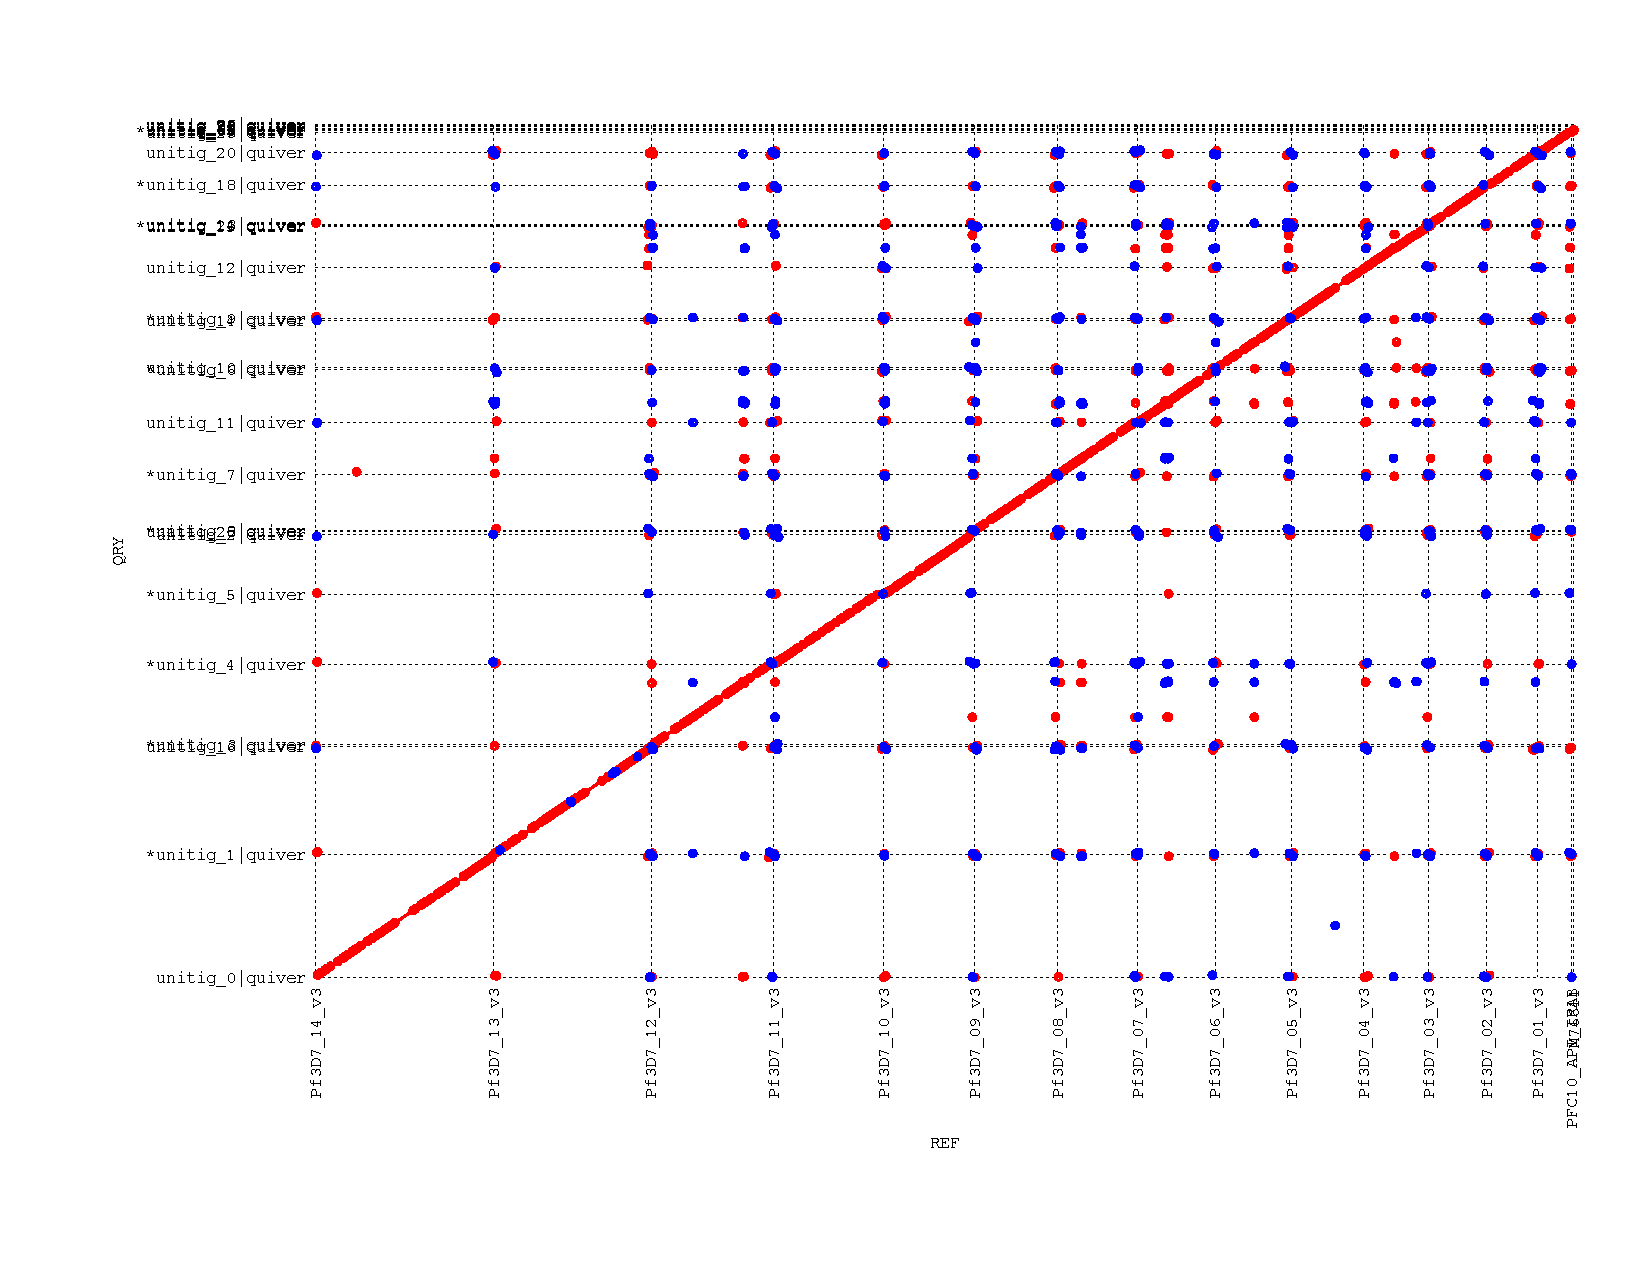
\includegraphics[width=\textwidth]{36F11dotplot}
  \caption{Alignment of contigs from PG0443-C to 3D7 reference assembly, with sequences from reference and draft assembly on the x and y-axis, respectively.  Each contig from the draft assembly is represented by a line segment terminated at either end with circles.  Red denotes forward alignment of contigs to the reference, blue denotes reverse alignment.}
  \label{fig:valdotplot}
\end{figure}

Having established the performance of the instrument and assembler in providing a viable assembly for a \textit{P. falciparum} isolate, we turned our attention to the validation sample from the 803xGB4 cross, PG0446-C.  We aligned the isolate's assembly to the 3D7 reference sequence using MUMmer, shown in Figure \ref{fig:valdotplot}.  Note that compared to the PG0051-C isolate, the validation isolate has much more off-diagonal activity, particularly towards the telomeres.  This is to be expected.  While the core genome between isolates is expected to be relatively stable, tremendous immune pressure has forced the antigenic repertoire to diversify rapidly.  These genes, primarily located in the subtelomeric regions, are the regions that land off-diagonal, indicative of the extensive recombination and mutation history.

We relabelled and reoriented each contig as necessary based on the alignment so as to more easily establish genomic positioning of events during analysis.  The assignments and orientation were further validated by transferring 3D7 gene model annotations onto the PG0446-C assembly by aligning each exon with \texttt{bwa mem}, operating under the assumption that the core genome is reasonably stable between isolates and that properly labelled and oriented contigs will yield exon alignments that match orientation and approximate positioning between the two assemblies.  Figure \ref{fig:loadGff} shows an example for chromosome $1$.  The vertical offset of all points is due to the fact that the assembly length of chromosome $1$ in the PG0446-C assembly is longer than the reference length.  Only exons towards the telomeric ends of the chromosome are misplaced, evidently originating from chromosomes other than chromosome $1$.  All other chromosome $1$ exons are aligned with the expected position and orientation.

After chromosome identification, we observed a handful of contigs that could not be assigned a place in the nuclear genome.  After running each unplaced contig through BLAST, we discovered two long contigs (thousands of bp) and nearly perfect hits to various species in the \textit{Pseudomonas} genus.  Discovering this contamination in the PacBio assembly and the Illumina samples strongly suggests the samples are contaminated at the source, contributing to the inflated 803xGB4 assembly lengths.  We removed these contigs from our assembly.

\begin{figure}[h!]
  \centering
    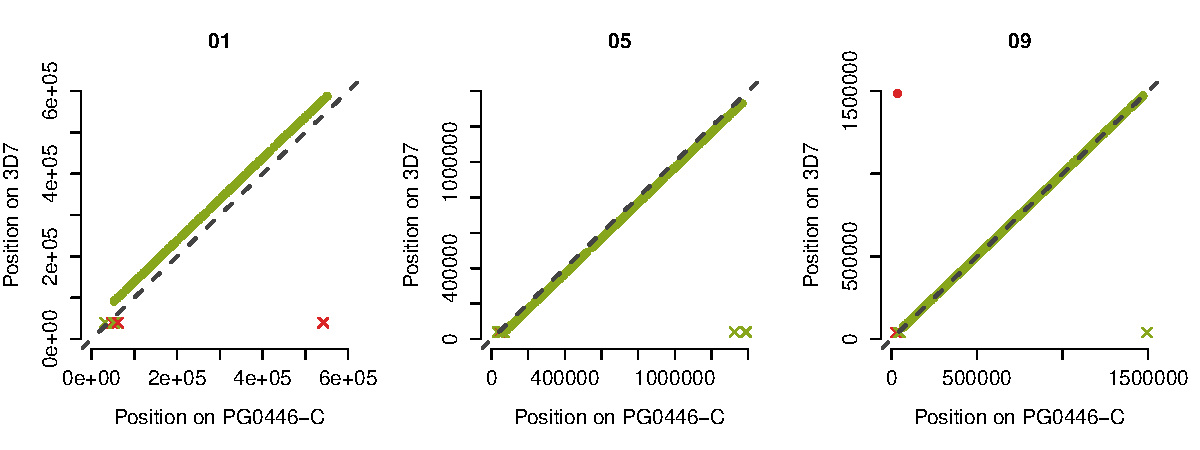
\includegraphics[width=\textwidth]{twochrs-1}
  \caption{Placement and orientation of exons from the reference assembly mapped to the PG0446-C assembly.  Chromosomes $1$, $5$, and $9$ shown.}
  \label{fig:loadGff}
\end{figure}

We verified sample identity by slicing the PacBio assembly into $1,000$ bp tiles (non-overlapping), aligning each tile to the 3D7 reference genome using \texttt{bwa mem}, and genotyping sites found to be variant in the MalariaGen 803xGB4 callset using the Genome Analysis Toolkit module, \texttt{UnifiedGenotyper} (specifying the genotype likelihood model to "SNP", ploidy to $1$, genotyping mode to "GENOTYPE\_GIVEN\_ALLELES", assuming default base quality scores should be $Q30$, and providing the 803xGB4 alleles from MalariaGen)\footnote{This procedure, while admittedly a bit indirect, provides vastly better results than genotyping the PacBio reads directly.  The assembly contains far fewer errors than the reads, even after error correction.  It is also much more straightforward than processing the MUMmer variant output, which uses a different file format to VCF, making comparisons cumbersome.}.  Chromosome $14$ is shown in Figure \ref{fig:showHaps}.  Note that while the PacBio sample's crossover pattern does appear to match that of PG0446-C, samples PG0445-C, PG0453-C, and PG0457-C also share the same pattern.  This common pattern is observed for these samples on all chromosomes.  These samples are almost certainly clones of one another.

\begin{figure}[h!]
  \centering
    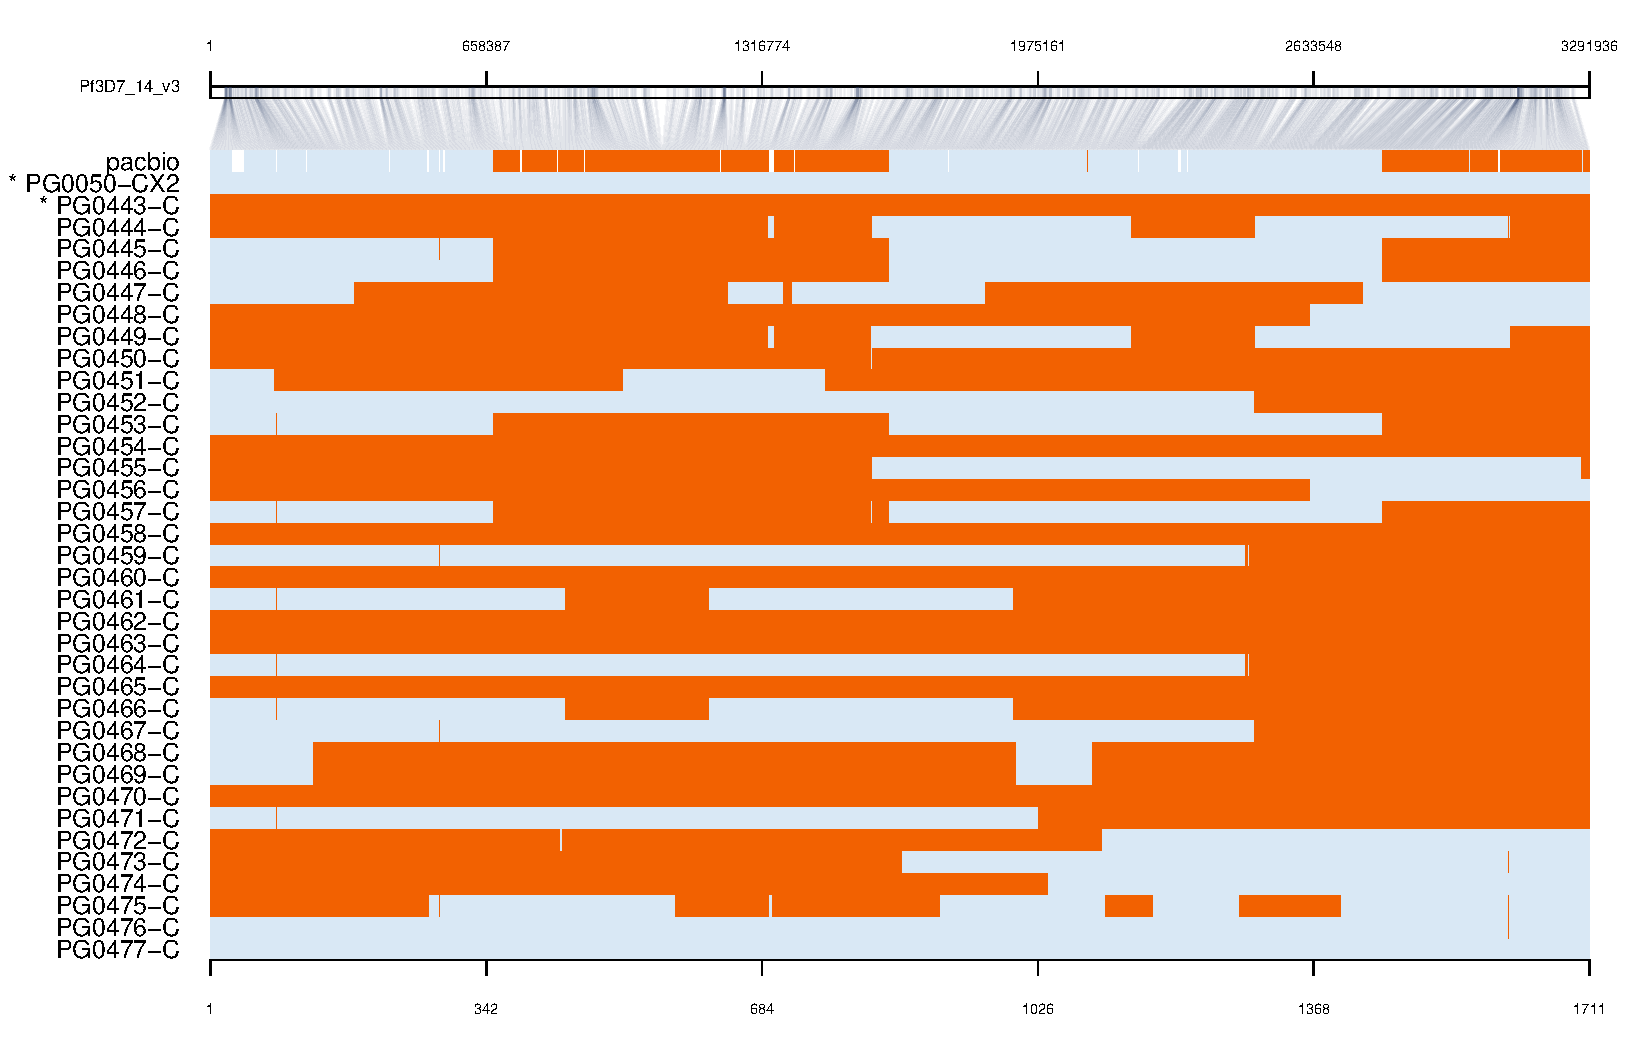
\includegraphics[width=\textwidth]{showHaps-14}
  \caption{Haplotype mosaic for chromosome $14$ in the 803xGB4 cross dataset.  Parental samples are identified with asterisks.  For remaining samples, alleles are color-coded according to the parent from which they are apparently inherited - orange for "mother" (PG0443-C, the 803 isolate), blue for "father" (PG0050-CX2, the GB4 isolate).  Missing data (sites where no genotype could be ascertained) are shown in white.  Bottom axis represents variant number.  Top axis represents variant position along the length of the chromosome.}
  \label{fig:showHaps}
\end{figure}

\section{Comparison to validation isolate}

\subsection{Verification of novel kmers}

As we have demonstrated that the PacBio assembly of the validation isolate is high-quality, novelty found in the Illumina dataset for the same sample can be verified by examining the PacBio isolate.  At the filtration levels of "all", "confident", and "trusted", initial processing of the Illumina data for 803xGB4 sample PG0446-C was found to have $28,904$; $17,069$; and $8,197$ novel kmers, respectively.  The PacBio assembly of the same sample recapitulates $1,639$; $802$; and $48$ novel kmers, respectively.  The discrepancies can be largely attributed to three (not necessarily independent) factors: an over-aggressive lower threshold for coverage, no upper threshold, and significant data contamination.

The first two points regarding coverage can be observed in Figure \ref{fig:covdists}a-c.  The leftmost panel shows a clear valley between the left end of the distribution (presumably sequencing errors, as they are so rarely observed in the dataset) and the first local maximum (likely real data).  In the middle panel, kmer coverage in PG0446-C decays more smoothly, and it is far less obvious as to where the lower threshold should be placed\footnote{It is worth mentioning that the PG0446-C sample, sequenced on more modern Illumina HiSeq 2000 platforms, likely enjoys a much lower sequencing error rate than the Illumina GAII used for PG0055-C, which contributes to our difficulty in automatically finding a reasonable coverage threshold.}.  In the rightmost panel, all novel kmers are shown, conditional to being present or absent in the PacBio assembly of the same sample.  Our automatically calulated threshold is clearly set too high, as it is slicing through the middle of the coverage distribution for novel kmers recapitulated by the PacBio dataset.

Furthermore, the rightmost panel shows a number of coverage outliers in the set of novel kmers that are not present in the PacBio dataset.  While their source is not immediately apparent, it is clear they have a large contribution to the set of novel kmers we examine; $1,057$ kmers present in the Illumina dataset but absent in the PacBio dataset were found to be high coverage outliers ($> 100x$).

\begin{figure}[h!]
  \centering
    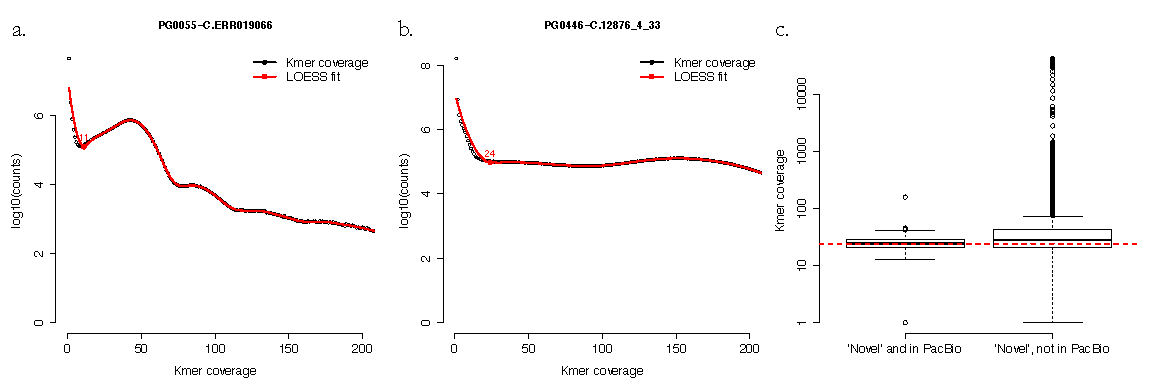
\includegraphics[width=\textwidth]{covdists}
  \caption{a. Kmer coverage in a 3D7xHB3 sample, with LOESS curve and calculated lower threshold at curve's first local minimum shown in red.  b. Kmer coverage in the 803xGB4 sample, PG0446-C, with LOESS curve and calculated lower threshold at curve's first local minimum shown in red.  c. Kmer coverage distributions for all novel kmers in PG0446-C, conditional on the kmer being present or absent in the PacBio assembly.  Calculated lower threshold from panel b shown as red dotted line.}
  \label{fig:covdists}
\end{figure}

We investigated other potentially erroneous novel kmers: putative novel kmers absent from the PacBio assembly and with coverage between $10x$ and $74x$.  We discovered many of these novel kmers exist in branches that either never connect with the graphs of the parents (we refer to these as "orphan" branches, Figure \ref{fig:orphans}a), or connect suspiciously amidst a number of putatively novel kmers rejected by the contamination checks (we refer to these as "bushy-tailed" branches, Figure \ref{fig:orphans}b).  Both appear to be symptoms of unrecognized contamination, owing to the fact that the BLAST database is not (and can never be) complete.  In attempting to remove any contribution to the graphs from non-target sources, it is insufficient to discard only the kmers that appear in the BLAST database.  Sequencing centers will always be sequencing new organisms, and the contents of the BLAST database will necessarily lag behind.  Discarding orphan branches is straightforward, but incompletely treats the problem; the bushy-tailed branches erroneously connect with the parental graphs and must be removed as well.

Finally, we discovered a substantial source of erroneous novel kmers stemming from "overcleaning", an issue wherein some kmers representing true genomic sequence are mistaken for sequencing error and removed from the graph via the assembler's error-cleaning or error-correcting process.  When this occurs in the parents but not the child (often due to coverage fluctuations), a kmer can appear to be "novel".  To mitigate this issue, we inspect the child's cleaned graph and the parents' dirty graphs.  However, a region of low coverage can also be flanked by regions of \textit{no} coverage; there are many kmers that are likely present in the parental genomes, but unobserved by chance.

\begin{figure}[h!]
  \centering
    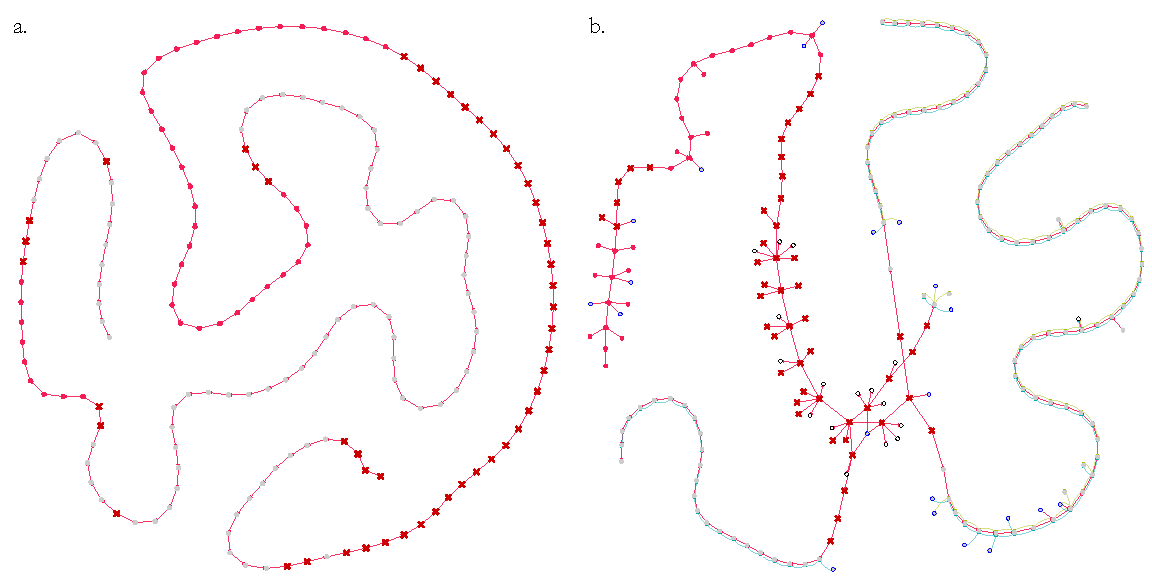
\includegraphics[width=\textwidth]{orphans}
  \caption{Local subgraphs in the Illumina data for PG0446-C near novel kmers that are absent in the corresponding PacBio assembly.  Red circles denote "trusted" novel kmers (those that passed our initial coverage and contamination checks).  Red crosses indicate "untrusted" novel kmers (those that passed our initial coverage check but failed the contamination check).  a. An "orphan" branch: a series of novel kmers not connected to the parental graphs.  b. A "bushy-tailed" branch: a series of novel kmers that appear to connect to everything, including the parental graphs, by chance.}
  \label{fig:orphans}
\end{figure}

To resolve these issues, we implemented a filtering solution for novel kmers in four parts.  First, we implemented a manual procedure for specifying coverage limits, selecting a lower limit of $10x$ and an upper limit of $74x$.  Next, we implemented software to explore the trio graph starting at confident novel kmers rejected by the contamination filter using our condition-limited depth first search software.  Explored branches containing novel kmers that are on the same branch as rejected kmers are similarly tagged for rejection.  Third, we explore the trio graph starting with remaining confident novel kmers.  If the explored subgraph does not connect with the parental graphs in any way, the kmers in the branch are marked for rejection and removed from further consideration.  Finally, we examine contigs with "overcleaned" novel kmers (i.e. any kmer that would be considered novel by comparing to the cleaned parental graphs, but is subsequently denied this label after examining the dirty parental graphs).  Novel kmers found on the same contig are considered tainted and removed from consideration.  Any putatively novel kmer surviving this battery of tests is considered "filtered".

The results of our novel kmer filtering are shown in Figure \ref{fig:novelfilter}.  $95$ kmers survive our battery of filters to be considered truly novel sequence in the genome of the PG0446-C child.  We called DNMs in the Illumina data using our graph-based calling software and discovered three events: two SNPs ($47$ kmers each) and a single kmer occurring in a repetitive region of a telomere; the precise nature of this single-kmer event is not clear.  The PacBio dataset contains $51$ novel kmers, $48$ of which overlap our calls (one SNP and the unknown event).  The other $47$ kmers from the second SNP are not present in the PacBio assembly.  However, manual inspection reveals this SNP to be polymorphic, possibly indicating a \textit{de novo} mutation that has occurred in the sample during mitotic divisions that has not yet reached fixation in the sequenced population of cells.  It is likely that the event (shown in Figure \ref{fig:pacbiohetsnpigv}) is a true variant, absent in the PacBio assembly as the Celera assembler is forced to make a choice between which allele to retain in the haploid assembly.  The presence of the alternate allele in the uncorrected PacBio read strongly suggests this is event is real and its absence from the assembly is an artifact of the assembler's bubble-popping procedure.  The remaining $3$ kmers from the PacBio dataset are not called in the Illumina data as they are low coverage (all at $1x$ coverage, all low complexity sequence, possibly representing recurrent sequencing errors in both the PacBio and Illumina data).

\begin{figure}[h!]
  \centering
    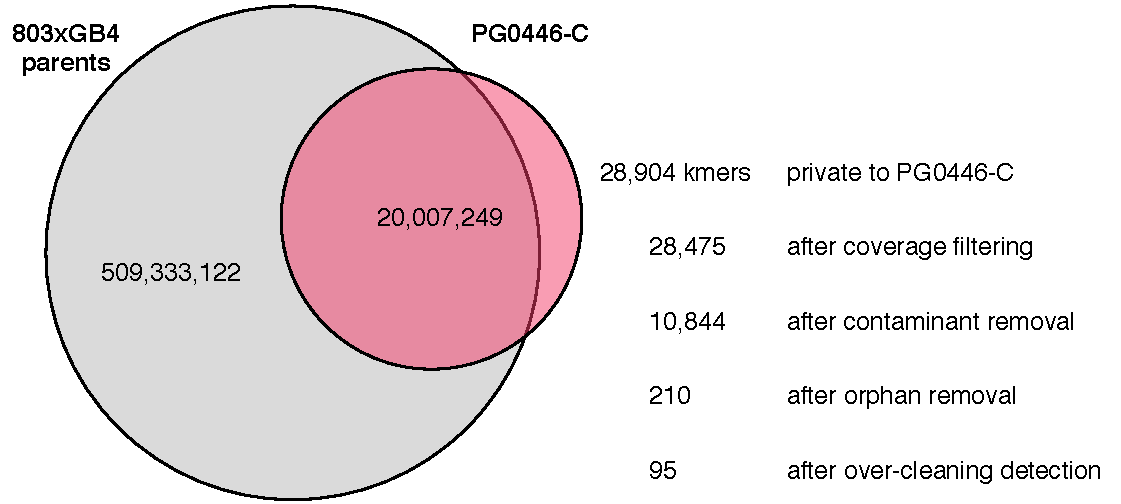
\includegraphics[width=\textwidth]{novelfilter}
  \caption{The results of filtering kmers private to the PG0446-C child }
  \label{fig:novelfilter}
\end{figure}

Based on the kmer recovery results listed above, our sensitivity to novel kmers is between $94\%$ and $100\%$ (depending on whether the $3$ missed kmers are considered truly novel kmers or sequencing errors), and specificity is greater than $99\%$.  Both SNPs and the unknown third event are recovered successfully.  The two SNPs are shown in Figures \ref{fig:pacbiohomsnpigv} (A to G, $13:2,032,381$) and \ref{fig:pacbiohetsnpigv} (C to T, $14:1,396,035$, a non-synonymous substitution resulting in a T to I amino acid change in \textit{PF3D7\_1433900}, a protein kinase).  Figure \ref{fig:weirdsinglenovelkmercomp} shows the third, unknown event.

\begin{sidewaysfigure}[h!]
  \centering
    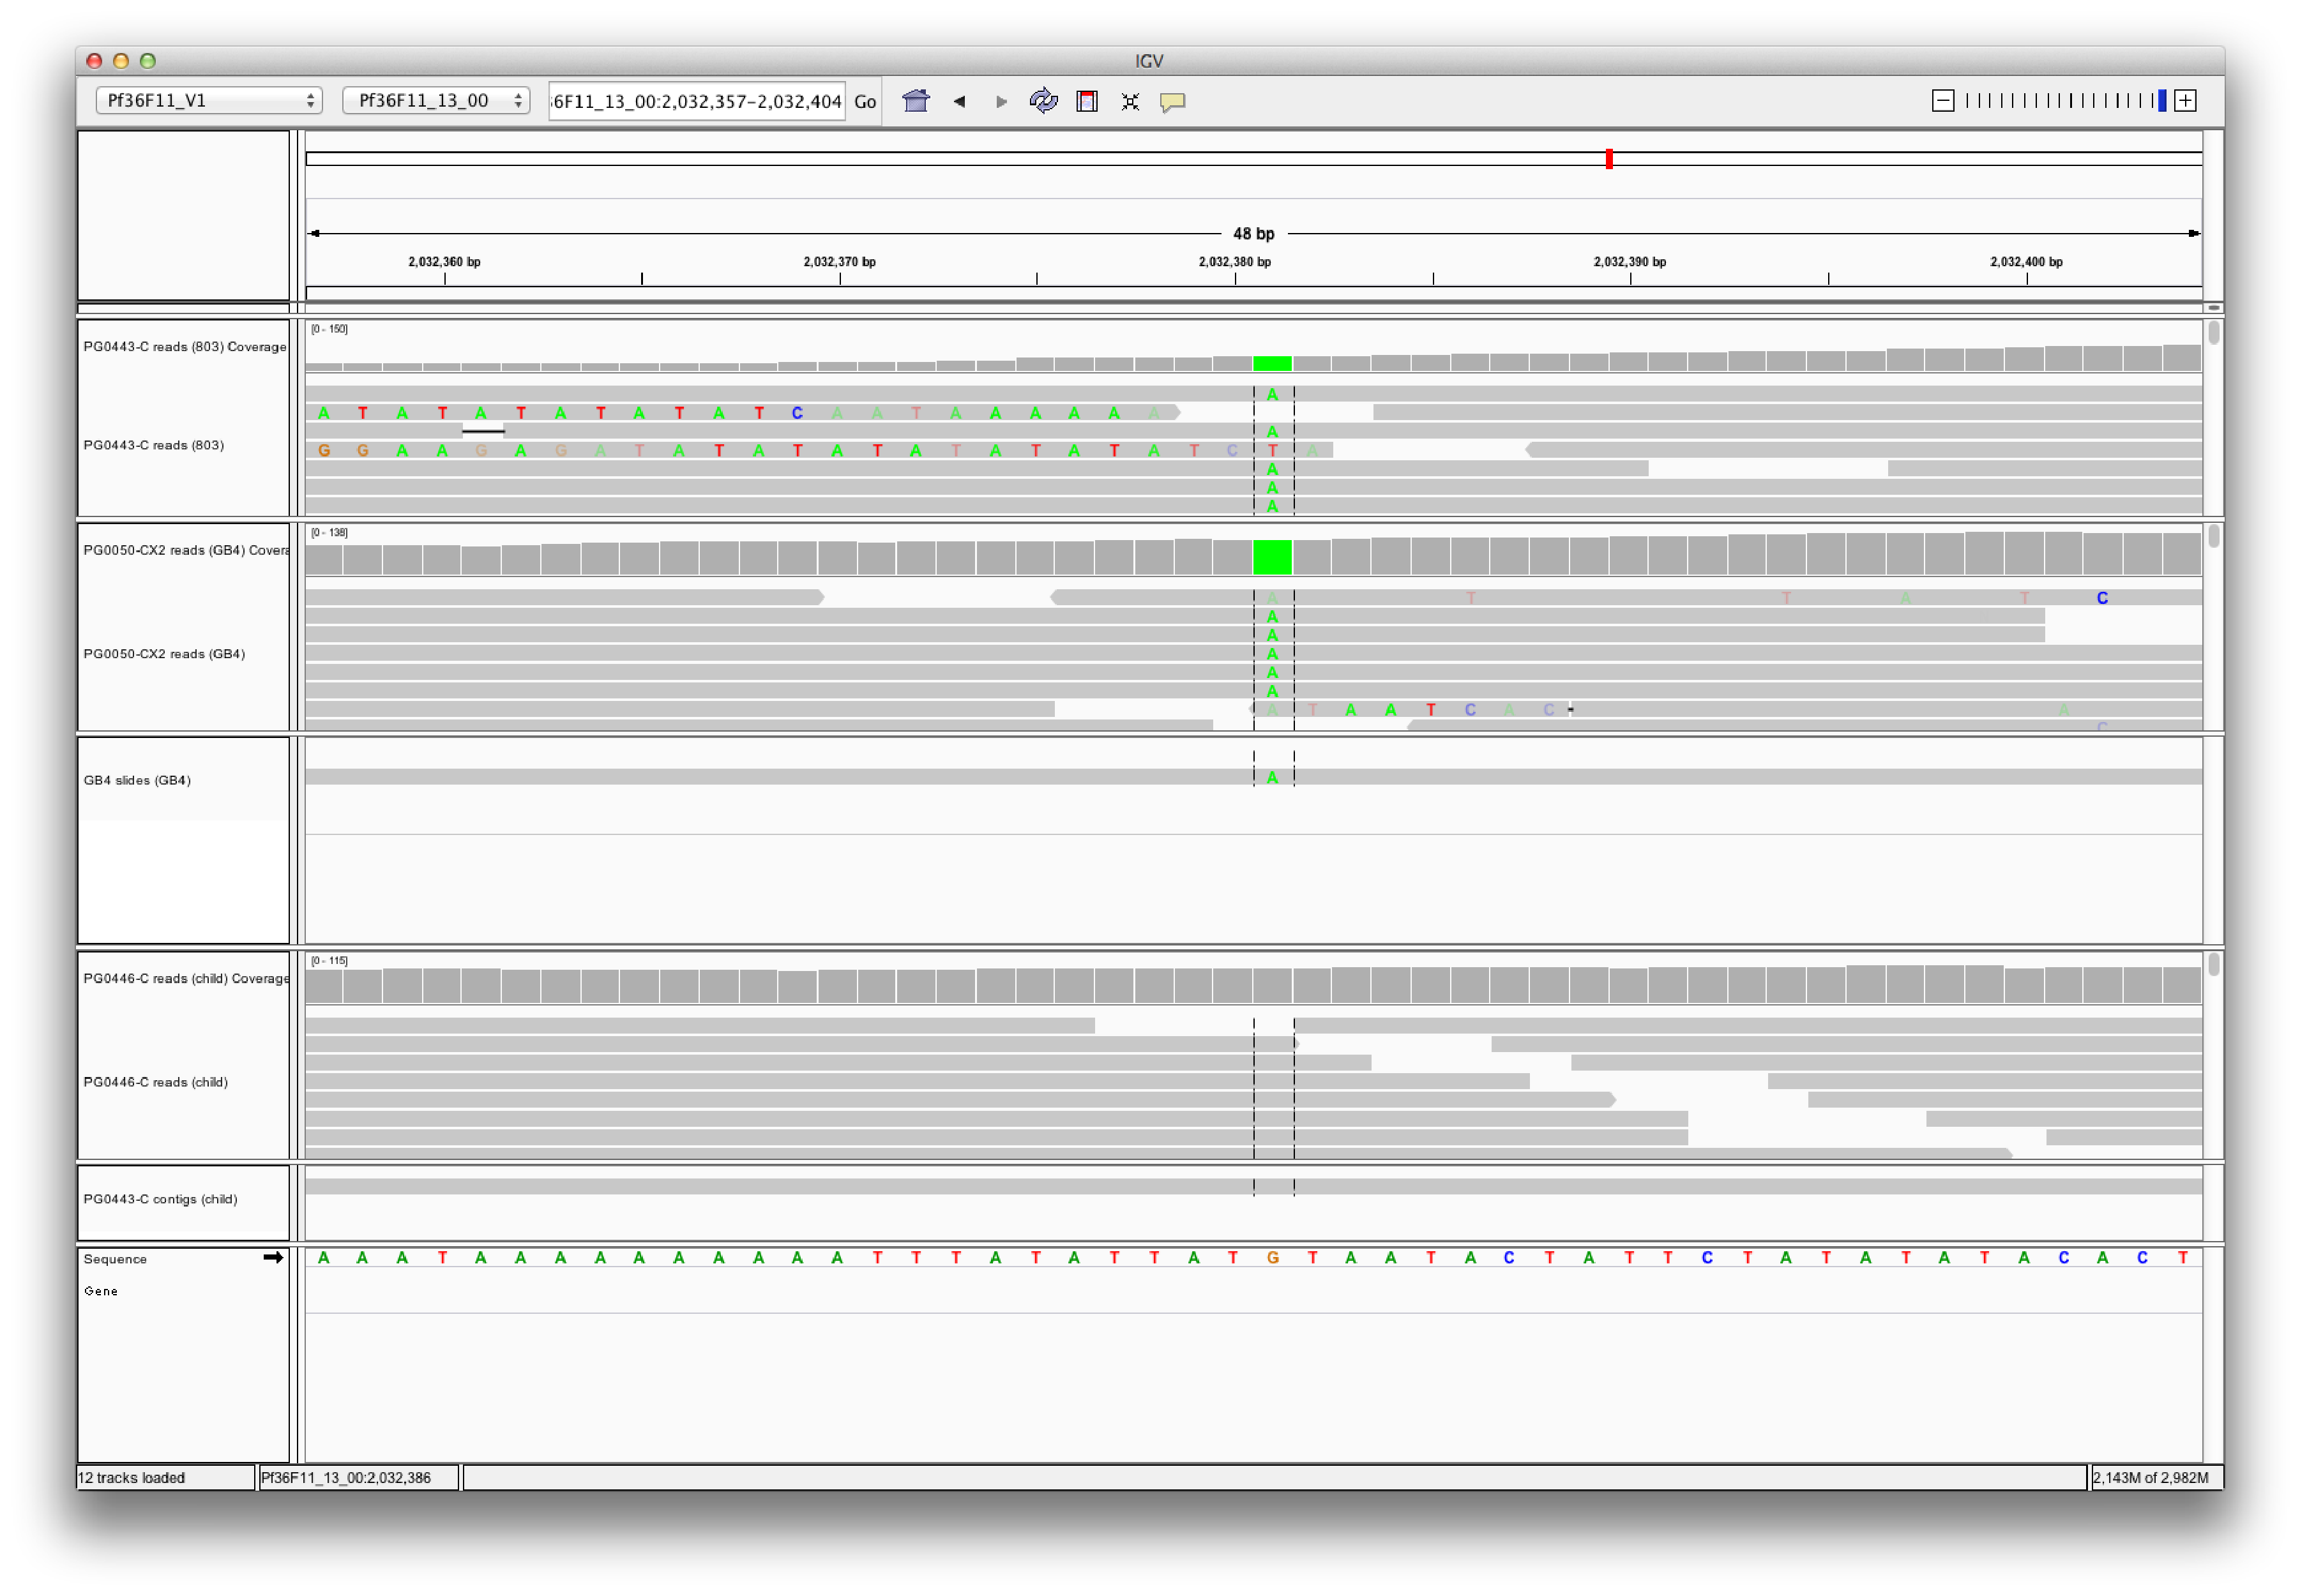
\includegraphics[width=\textwidth]{pacbiohomsnpigv}
  \caption{IGV screenshot of an A to G SNP, showing reads and assembly information for the trio, aligned to the PacBio PG0446-C assembly.  Top panel: 803.  Middle two: GB4 reads and PacBio assembly (sliced to facilitate alignment).  Lower two: PG0446-C reads and contig containing the variant in question from the a. panel.}
  \label{fig:pacbiohomsnpigv}
\end{sidewaysfigure}

\begin{sidewaysfigure}[h!]
  \centering
    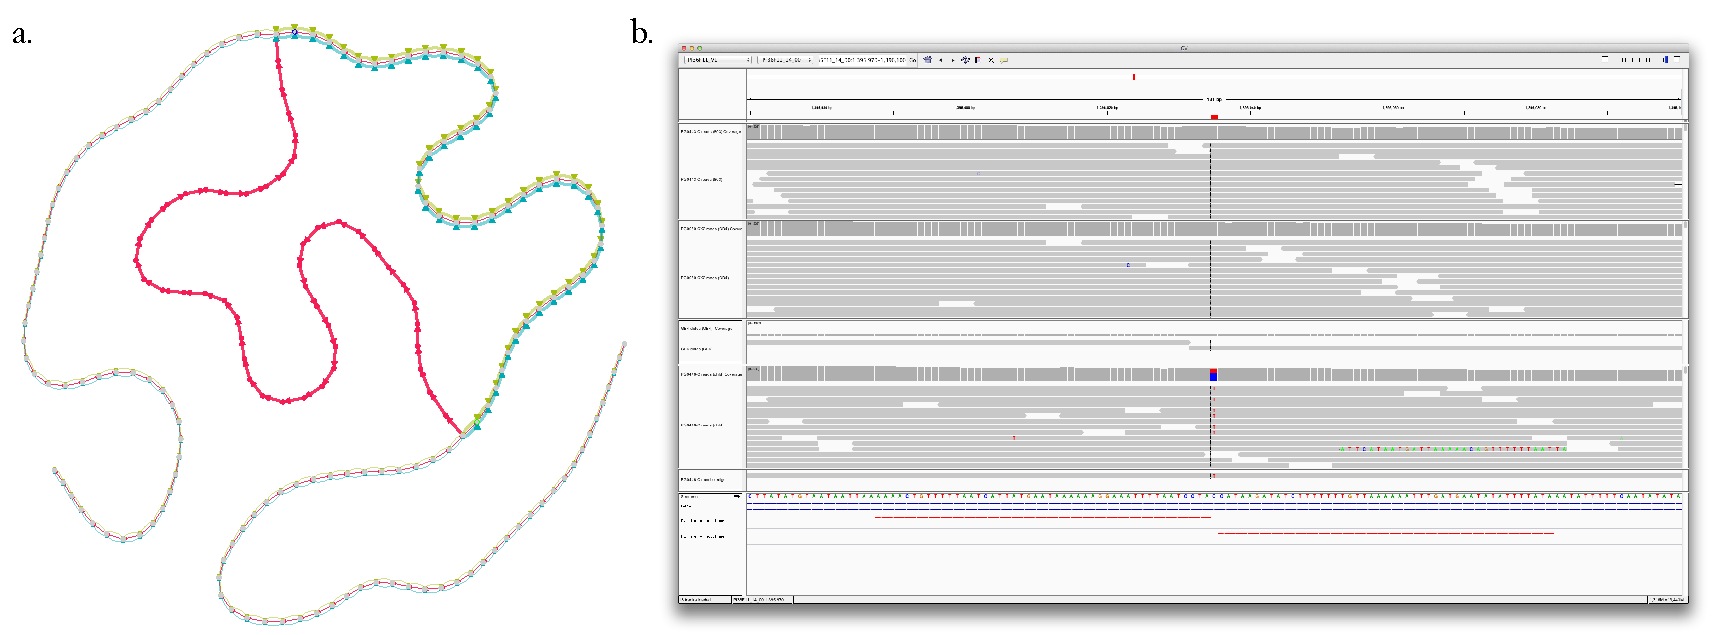
\includegraphics[width=\textwidth]{fpcomp}
  \caption{A C to T SNP that has likely not reached fixation in the sequenced population of ostensibly clonal parasites.  a. Local subgraph at the site, wherein the child's graph contains paths that traverse the series of novel kmers as well as the parental kmers, indicating polymorphic status.  b. IGV screenshot of the site showing reads and assembly information for the trio, aligned to the 3D7 reference genome.  Top panel: positions of the called variants in the reference-basde analysis.  Second panel: PG0443-C (803).  Third: PG0050-CX2 (GB4).  Fourth: PG0446-C (child).  Fifth: Uncorrected PacBio reads from PG0446-C.  Bottom: gene model track from PlasmoDB $9.0$.  Stacked barplots above tracks indicate the proportion of reads supporting each allele.}
  \label{fig:pacbiohetsnpigv}
\end{sidewaysfigure}

\begin{sidewaysfigure}[h!]
  \centering
    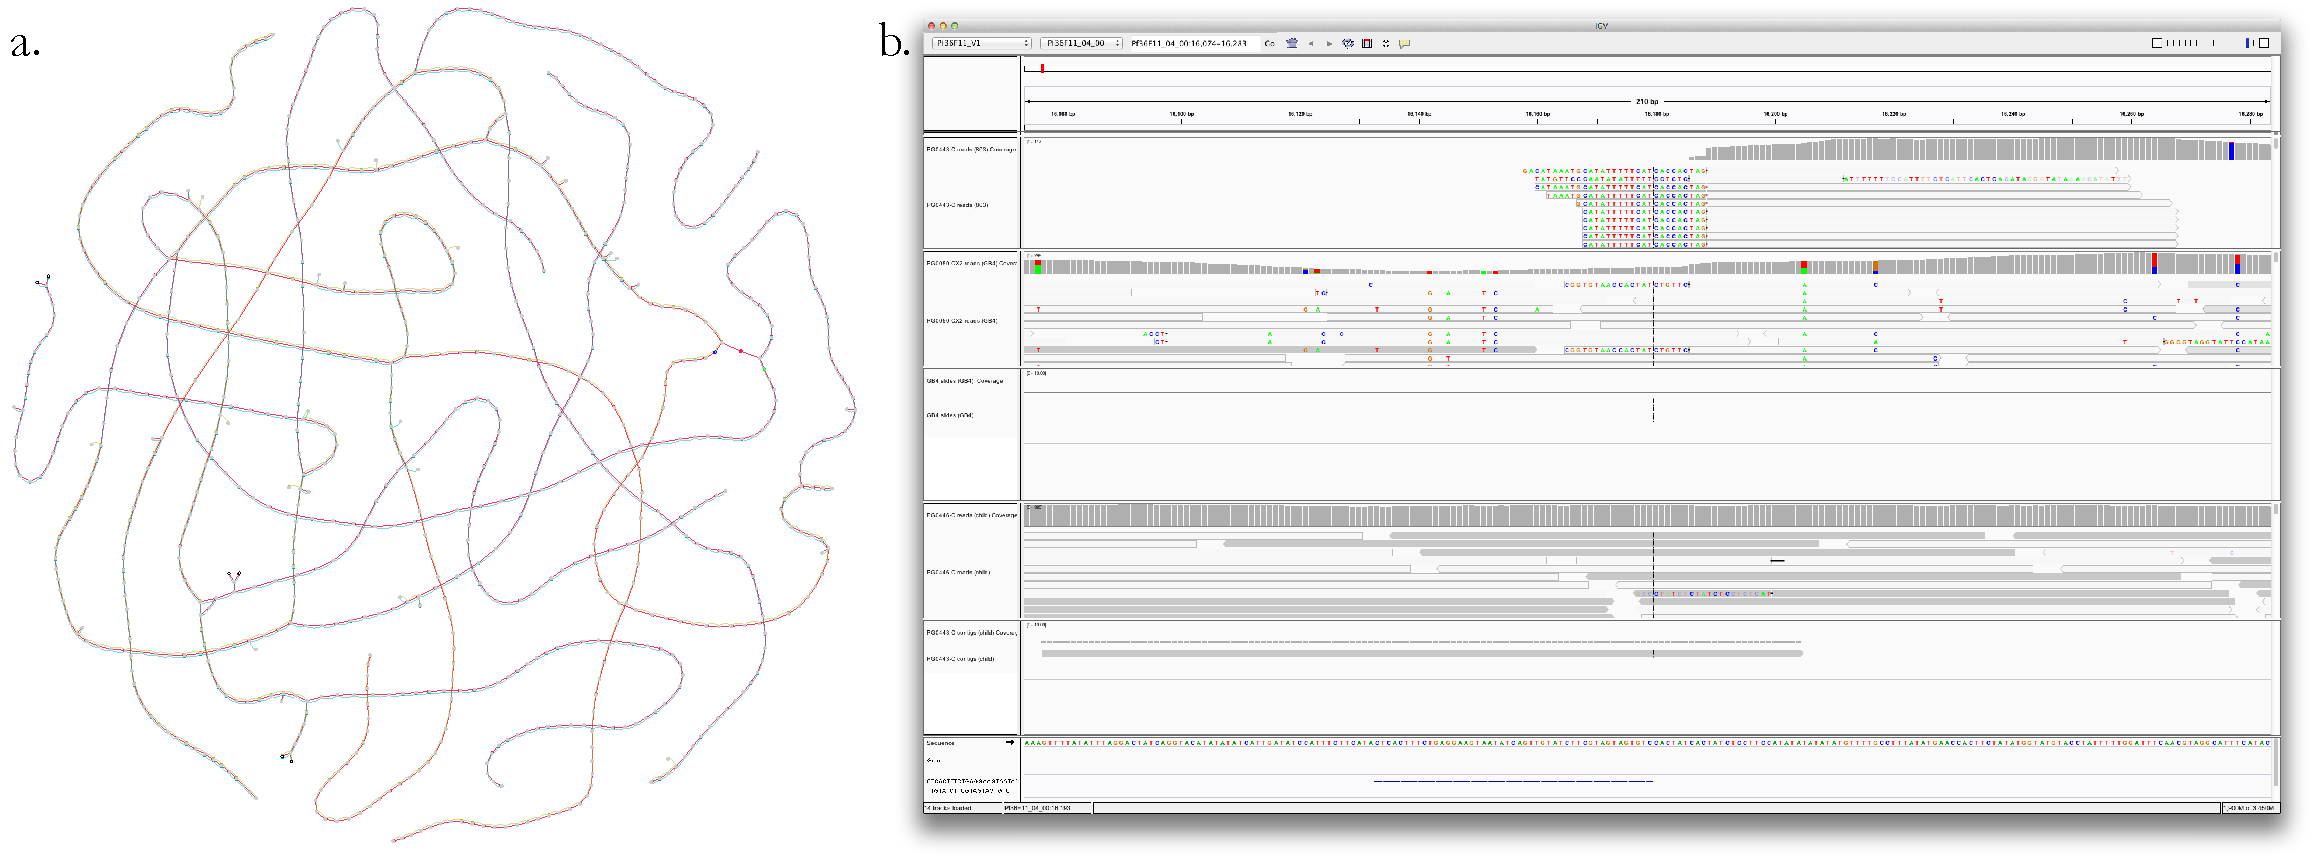
\includegraphics[width=\textwidth]{weirdsinglenovelkmercomp}
  \caption{A strange event involving a single novel kmer.  a. Local subgraph at the site; the novel kmer in question is depicted as a filled red vertex in the right side of the image.  b. IGV screenshot of the site showing reads and assembly information for the trio, aligned to the PacBio PG0446-C assembly.}
  \label{fig:weirdsinglenovelkmercomp}
\end{sidewaysfigure}

\subsection{Comparison to reference-based analysis}

We sought to determine our relative ability to detect DNMs accurately compared to that of the reference-based analysis.  As the release version of the MalariaGen callset purposefully excluded \textit{de novo} mutations (attempting to minimize Mendelian error rates to ensure high confidence in the inherited variation callset), we set about processing the Illumina data from the PG0446-C trio (PG0443-C (803), PG0050-CX2 (GB4), and PG0446-C) ourselves.  Reads were aligned with \texttt{bwa mem} to the 3D7 reference genome, release $9.0$ from PlasmoDB.  PCR duplicates were marked with the \texttt{MarkDuplicates} program from the Picard suite; these marked reads were subsequently ignored in downstream processing.  A list of genomic regions with reads appearing to span indels were discovered using the GATK's \texttt{RealignerTargetCreator} module (supplemented by MalariaGen's 803xGB4 calls as additional candidate regions to consider).  We subsequently ran the GATK's \texttt{IndelRealigner} to perform the local realignments on these candidate regions.  We recalibrated base quality scores using the GATK's \texttt{BaseRecalibrator} tool, once again supplying the MalariaGen calls as sites to ignore when computing the data error model.  Variants were called across the PG0443-C, PG0050-CX2, and PG0446-C samples simultaneously using the GATK's \texttt{HaplotypeCaller} module, which performs local \textit{de novo} assembly to determine the haplotype sequence at so-called "active sites", windows of the genome detected to harbor some sort of variation.  For each approach, we specified a ploidy of $1$.  SNPs and indels were filtered separately using the GATK's \texttt{VariantRecalibrator} tool, supplying the MalariaGen calls as training data.  We set the desired truth sensitivity to $99\%$ (i.e. requesting that the recalibration tool learn filter thresholds such that at least $99\%$ of the MalariaGen calls were recapitulated).  Finally, we isolated putative DNMs by selecting sites confidently called in all three samples, where the genotype of the child differed from that of mother and father, requiring confident genotypes in all three samples (i.e. $GQ > 90$), and sufficient allele depth in all three samples (i.e. $DP > 20$).

Callset metrics are presented in Table \ref{tbl:gatkmetrics}.  Note that while MalariaGen chose to include calls only in the so-called "core" region of the genome (comprising $20.7$ Mbp of sequence), we have included the accessory genome in our callset as well (the remaining $2.5$ Mbp of genomic sequence spanning telomeric, subtelomeric, pericentromeric, and other hypervariable loci).  For a fairer comparison, we have partitioned the calls into the core and accessory regions.  Furthermore, in addition to the monomorphic sites one expects to see in a haploid genome for a \textit{de novo} variant that occurs during meiosis or in one of the gametocytes, the trio contains thousands of polymorphic sites ($23,004$ sites where the reference allele and alternate allele have non-zero coverage, $4,364$ with reference and alternate allele coverage greater than $10x$).  Both the accessory genome and polymorphic sites are easily removed.  However, given that our graph-based approach is theoretically able to access the accessory genome and that we saw at least one polymorphic site in our graph-based \textit{de novo} mutation callset, we chose not to exclude these sites at this stage.

\begin{table}[]
\centering
\caption{Callset metrics in the PG0446-C sample of the trio}
\label{tbl:gatkmetrics}
\begin{tabular}{@{}rrrrrr@{}}
\toprule
\multicolumn{1}{l}{}           & All      & In MalariaGen & Not in MalariaGen & Core     & Accessory \\
\midrule
\multicolumn{1}{l}{SNPs}       &          &               &                   &          &           \\
\textit{all}                   & $28,613$ & $5,742$       & $22,871$          & $13,700$ & $14,913$  \\
\textit{de novo}               & $128$    & $0$           & $128$             & $7$      & $121$     \\
\multicolumn{1}{l}{Insertions} &          &               &                   &          &           \\
\textit{all}                   & $15,163$ & $4,543$       & $10,620$          & $12,540$ & $2,623$   \\
\textit{de novo}               & $38$     & $0$           & $38$              & $8$      & $30$      \\
\multicolumn{1}{l}{Deletions}  &          &               &                   &          &           \\
\textit{all}                   & $17,762$ & $5,160$       & $12,602$          & $15,123$ & $2,639$   \\
\textit{de novo}               & $30$     & $0$           & $25$              & $5$      & $25$      \\
\multicolumn{1}{l}{MNPs}       &          &               &                   &          &           \\
\textit{all}                   & $144$    & $0$           & $144$             & $65$     & $79$      \\
\textit{de novo}               & $0$      & $0$           & $0$               & $0$      & $0$       \\
\bottomrule
\end{tabular}
\end{table}

We identified $196$ potential \textit{de novo} variants in the PG0443-C sample using the reference-based \texttt{HaplotypeCaller} approach and the filters described above.  This is two orders of magnitude greater than the number of DNMs we found in the PacBio data.  As expected, much of this putative variation appears in the accessory compartments of the genome, owing to the massive divergence between the reference and sampled haplotypes.  However, even when we restrict our analysis to the core genome, we still find an order of magnitude more events than we expect in the graph approach.

We sought to establish the veracity of any of these putative \textit{de novo} events.  Assuming the child's underlying haplotype is the reference haplotype plus the variants discovered in that sample, we expected to find kmers spanning the DNMs to be present in the PacBio assembly, present in the clean graph of the child, and absent in the dirty graphs of the parents.  Revisiting Algorithm \ref{alg:all_subsets} from Chapter \ref{ch:motivation}, we combinatorically generated kmers spanning all \textit{de novo} variants and any nearby variants (including variants that were filtered out) that would affect the local haplotype.  $30,360$ such kmers were generated, $3,740$ of which are present in our PacBio draft reference for the child.  $3,547$ ($\approx 95\%$) of these kmers are present in the Illumina data for the child as well.  $3,500$ of these are present in the dirty graphs of the parents, suggesting that all associated events ($195/196$) are false positives.

The remaining $47$ kmers represent a single SNP: the clearly homozygous SNP on chromosome $13$ discussed in the previous section.  This is the only event recapitulated between the PacBio dataset and these calls.  However, we note that in selecting our coverage thresholds, we benefitted from prior knowledge.  The coverage in the 803 parent is approximately $30x$, while coverage in the GB4 parent and the child are in excess of $60x$; our depth filtering threshold was specifically chosen to recover this validated variant.  The SNP is shown in Figure \ref{fig:homlowcov}; the PG0443-C (803) panel shows the drop in coverage in the downstream intergenic region beyond PF3D7\_1350600.  In this region, sequence complexity drops sharply, dominated by runs of As and Ts.  Sequencing error may be accumulating in reads sampled from this region such that they fail to align back, thus contributing to the coverage falloff.  Raising the coverage threshold would of course remove more false-positives, but there is no \textit{a priori} reason to choose a threshold of $20x$ versus $30x$ (especially when average coverage in the 803xGB4 samples is around $200x \pm 100x$).

The polymorphic variant on chromosome $14$ is not present in the reference-based callset, owing to the fact that we instructed \texttt{HaplotypeCaller} to assume a ploidy of $1$.  If we genotype this site alone without the ploidy specification, we can recover the event.  However, removing the ploidy specification does not mean allowing any ratio of reference to non-reference alleles at a putative variant site.  Instead, the software simply defaults to a ploidy of $2$, which is not necessarily a correct assumption to make for our data.  The ploidy setting merely enables the caller to adjust its allele balance expectations, and revising it upwards increases the chance that the caller will accept sequencing error as variation.  Thus, removing the ploidy setting would necessarily increase the false-positive rate as well.

We visually inspected the alignments spanning the false \textit{de novo} events using IGV.  Many of these sites were seemingly polymorphic as well, in close proximity to one another, and in known high-diversity regions of the genome.  Figure \ref{fig:lotsosnps} depicts one such example of false-positives on chromosome $2$.  It is possible to begin adding heuristic filters to remove these events (e.g. rejecting events on allele balance, inter-marker distance, and the genomic compartment in which they are discovered).  However, there are two very good reasons not to do so.

First, consider the underlying cause of these artifacts.  The myriad inconsistencies between the Illumina reads for PG0446-C, the PacBio reads for the same sample, and the presence of many mapping quality $0$ reads, strongly suggests misalignment.  The true haplotype from which these reads are sampled are clearly not in the reference genome, but are similar enough that many reads map anyway, and the precise placement is a function of read length and repetitiveness of the sampled haplotype.  When we align reads from this region in the child to the PacBio reference for the child, we find that most map to chromosome $1$, not chromosome $2$.  Filters can only accomplish one thing: reject potential false-positives.  However, filters can do nothing to address the root issue: the reads were sampled from one region of the child's genome and aligned to a sample too genomically divergent in these loci to serve as a useful platform for comparison.  Application of such filters would necessarily require sacrificing any ability to say something meaningful about enormous diverse regions of the genome.

Second, consider what these variants in a haploid genome must represent: \textit{de novo} mutations that have occurred while the parasites have been in culture and have not reached fixation in the sample.  These events necessarily must have occurred during mitosis, as mutations incurred during meiosis or present in the gametocytes would appear in every read spanning the site.  Filtering any events based on allele balance would necessarily mean discarding every potential mitotic \textit{de novo} mutation\footnote{In a haploid genome, every true variant presenting as seemingly polymorphic must be a mitotic event, but as some mutations could have reached fixation in the sample, not every mitotic event will necessarily present as polymorphic.}.

\begin{sidewaysfigure}[h!]
  \centering
    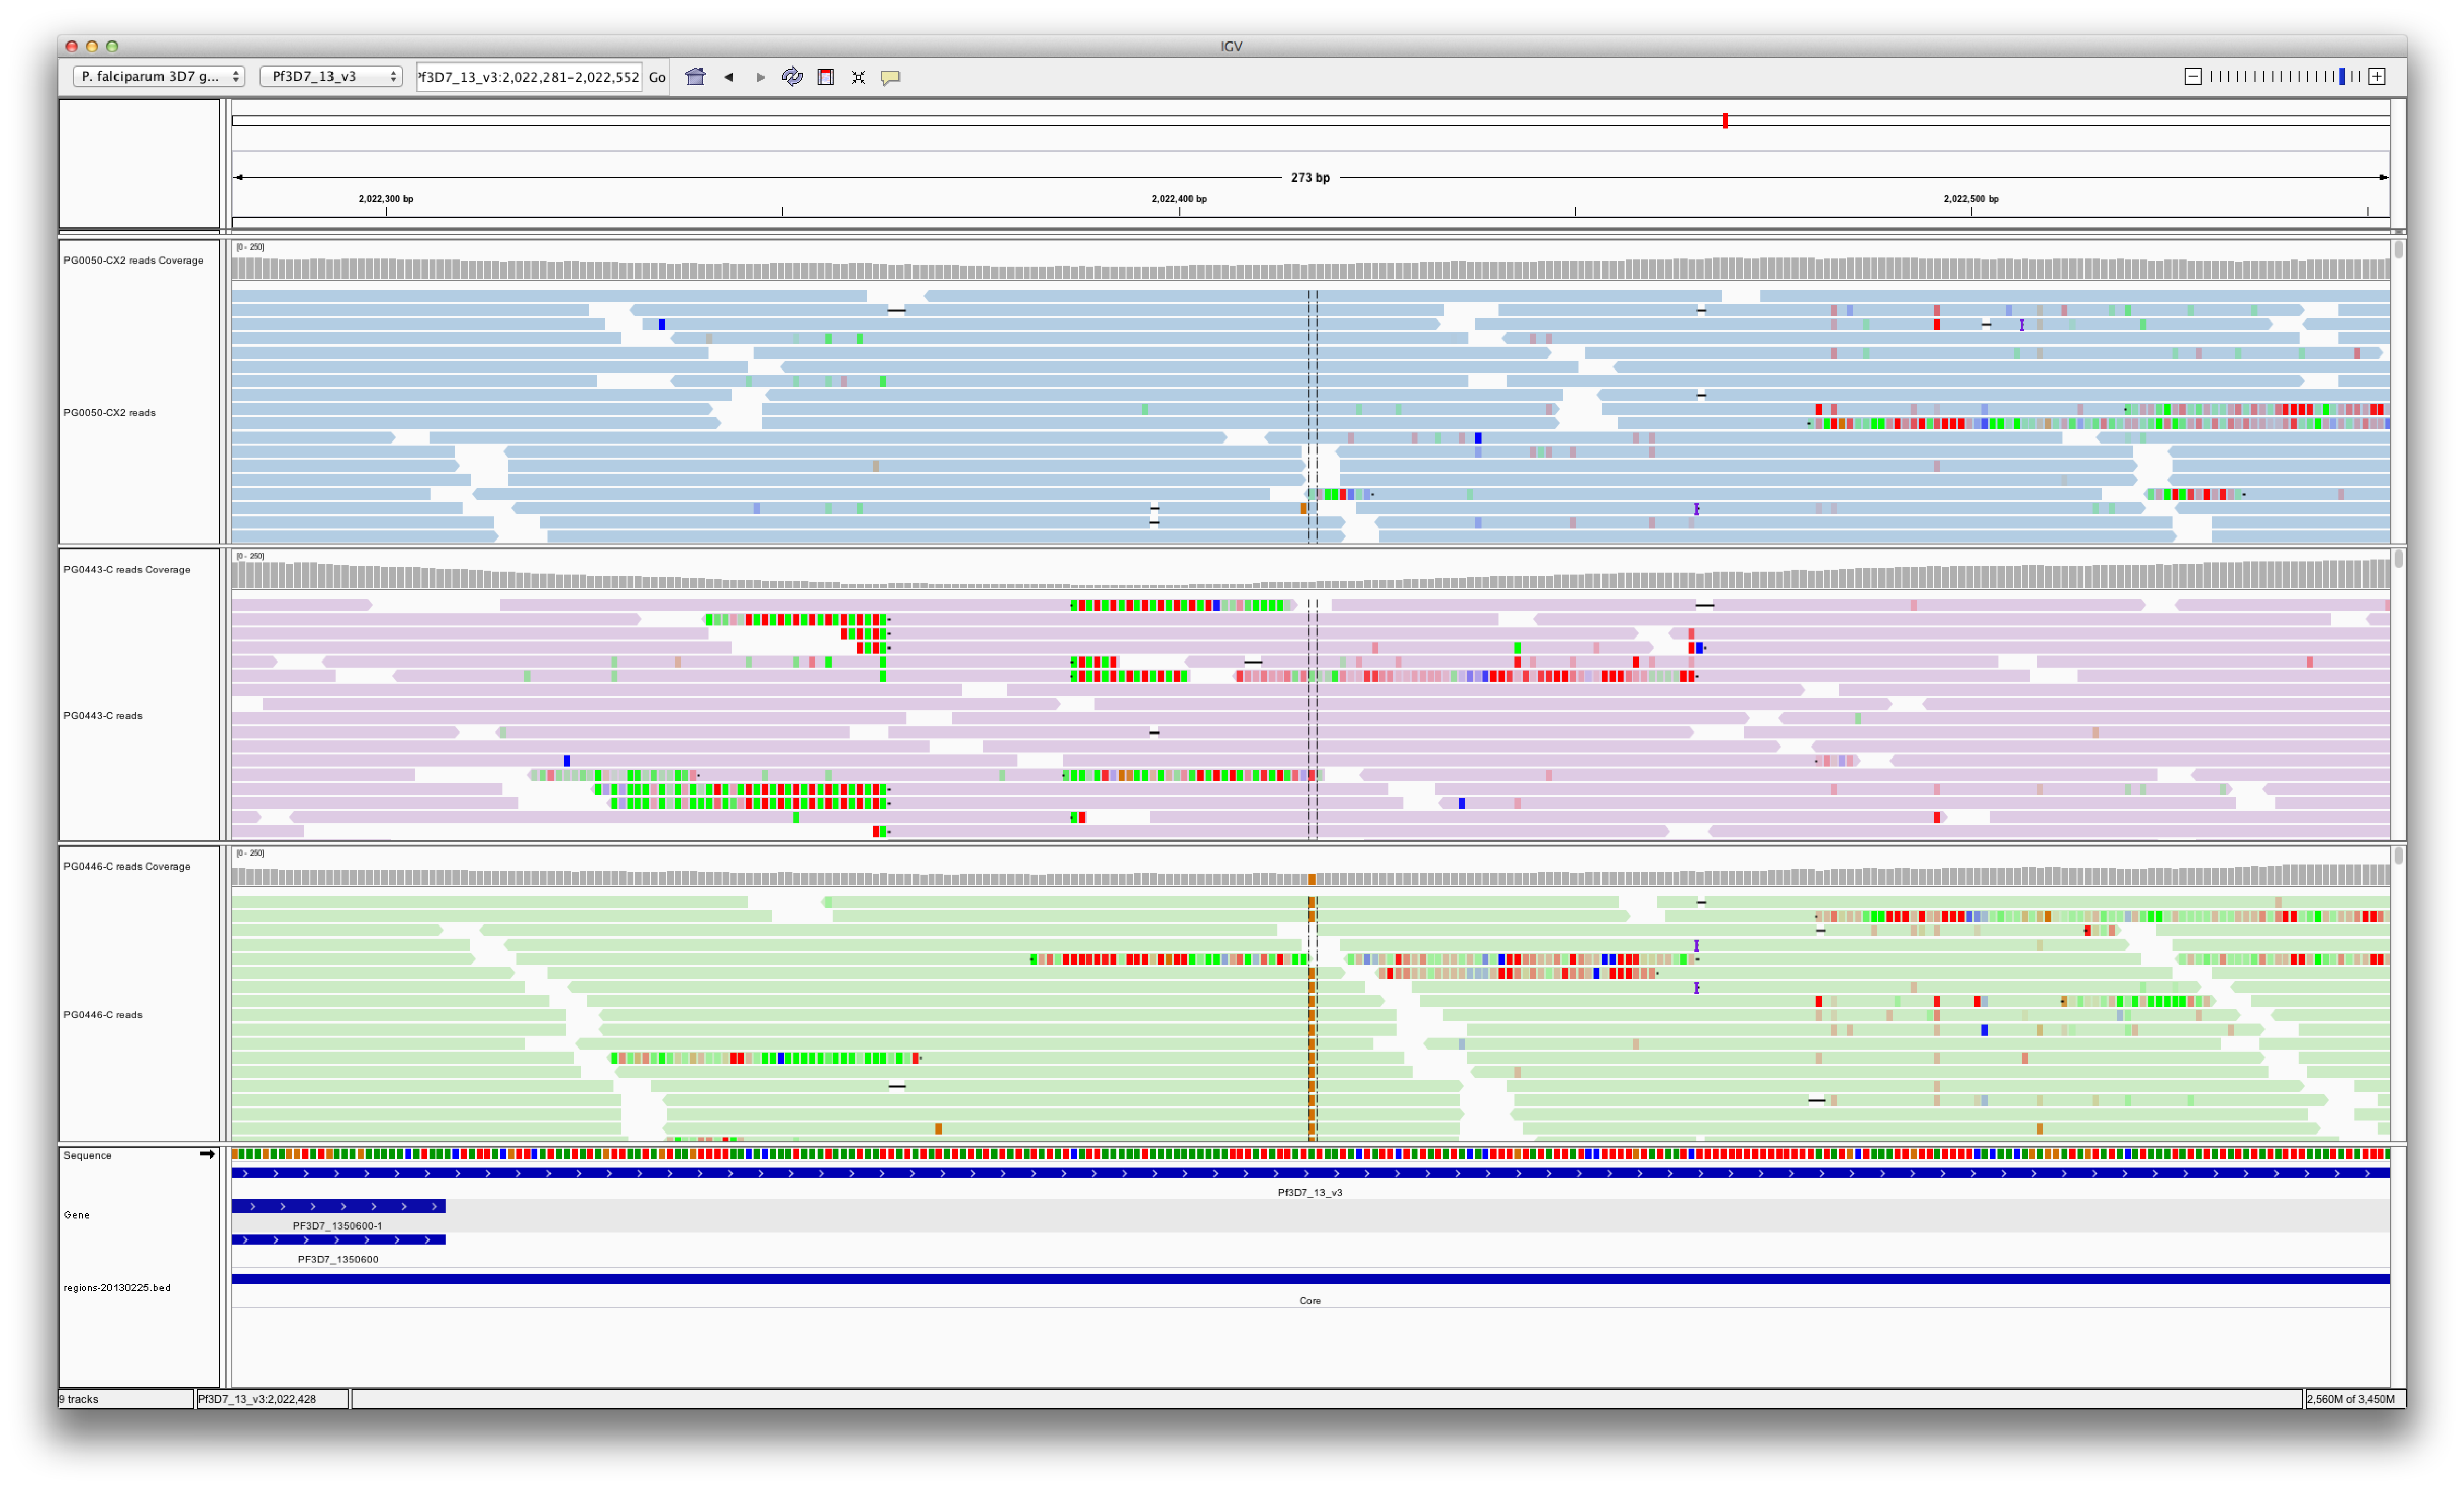
\includegraphics[width=\textwidth]{homlowcov}
  \caption{A validated \textit{de novo} SNP, recovered in the child amidst a great deal of sequencing error.  Top panel: PG0443-C (803).  Middle panel: PG0050-CX2 (GB4).  Lower panel: PG0446-C (child).}
  \label{fig:homlowcov}
\end{sidewaysfigure}

\begin{sidewaysfigure}[h!]
  \centering
    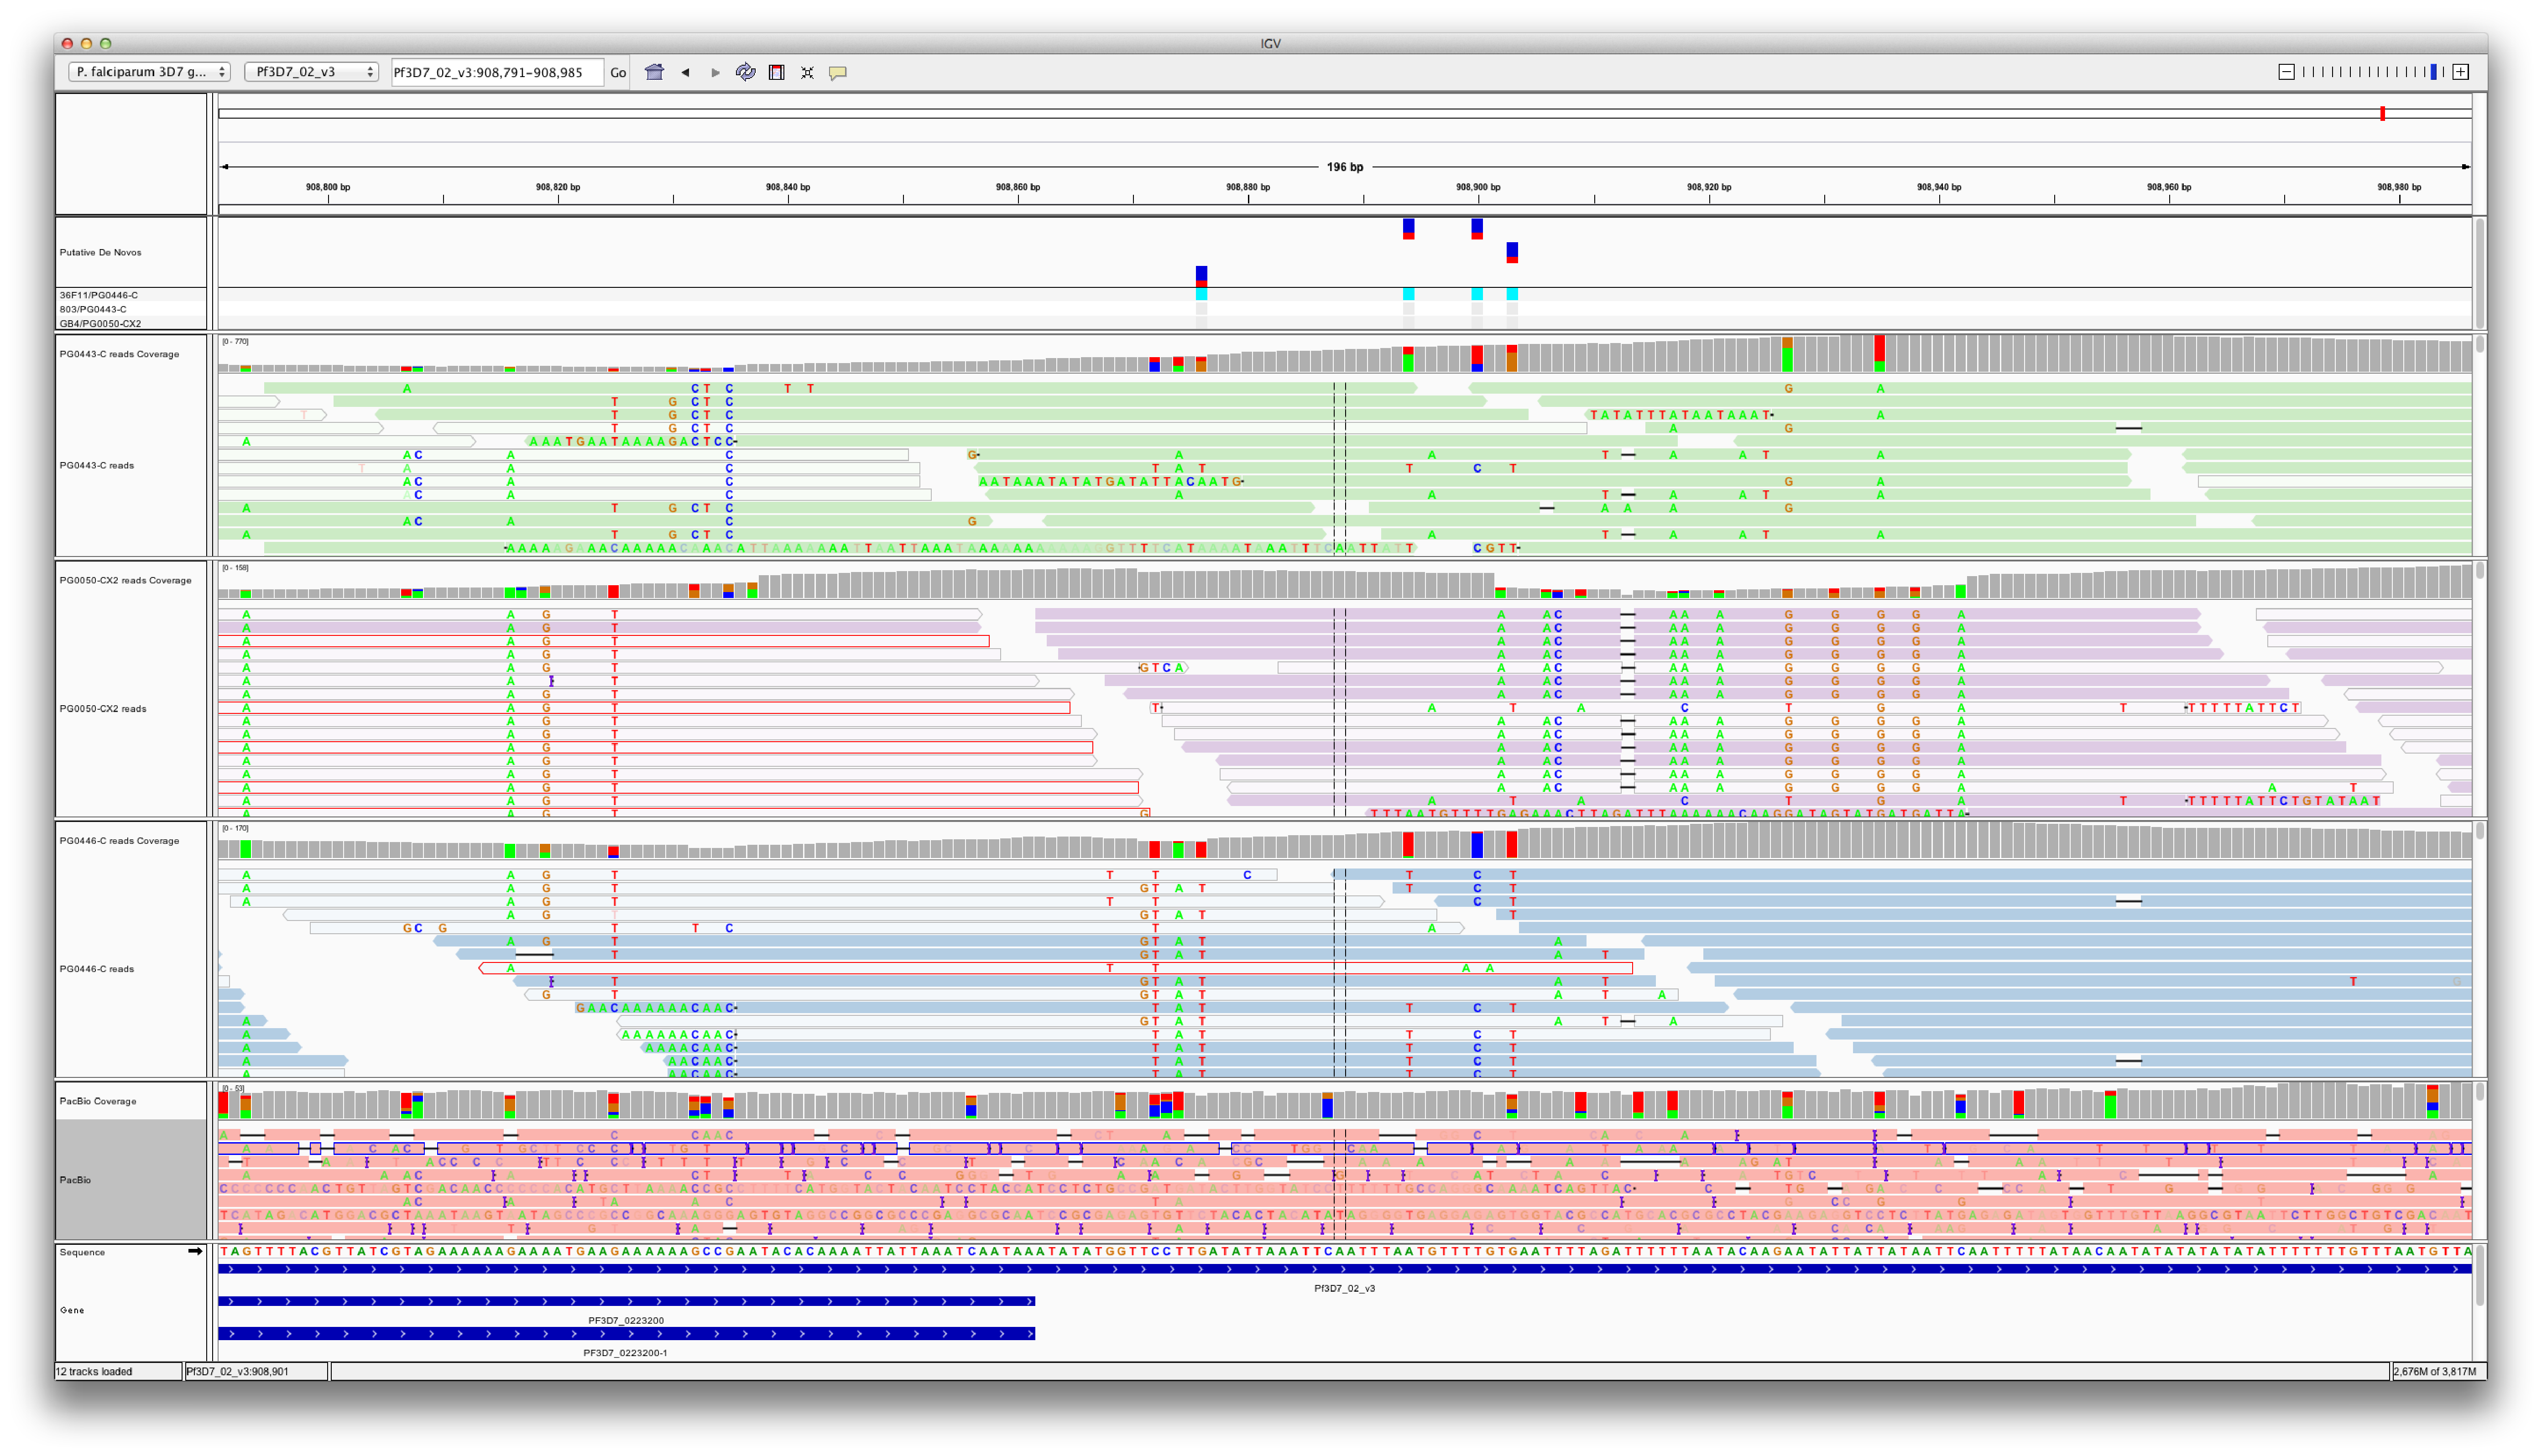
\includegraphics[width=\textwidth]{lotsosnps}
  \caption{False-positive \textit{de novo} variants in the 3' subtelomeric region of chromosome $2$.  Top panel: positions of the called variants in the reference-based analysis.  Second panel: PG0443-C (803).  Third: PG0050-CX2 (GB4).  Fourth: PG0446-C (child).  Fifth: Uncorrected PacBio reads from PG0446-C.  Bottom: gene model track from PlasmoDB $9.0$.  Stacked barplots above tracks indicate the proportion of reads supporting each allele.  Reads with ambiguous alignments are displayed in a lighter shade.}
  \label{fig:lotsosnps}
\end{sidewaysfigure}

\section{Summary}

Despite only having a single PacBio validation dataset, it has taught us a trmendous amount.  We have seen how the coverage filter we developed in Chapter \ref{ch:methods} is insufficient; we need to relax the lower bound in higher quality data, and we must add an upper bound to remove some repetitive noise.  We have also seen how contamination can have a profoundly negative effect on our list of novel kmers, filling the list with junk, forcing us to examine too many places in the genome graph, and inflating our measure of \textit{de novo} mutation sensitivity.  Our general purpose machinery for traversing the graph until a specified stopping condition is met enables us to explore the graph at these contaminating kmers and remove all connected novel kmers from consideration.  Effectively, they are tainted as being guilty by association.  With the inclusion of these filters, we finally demonstrate that our sensitivity and specificity in the test sample are essentially perfect, and that we can distinguish between both monomorphic events (presumably events that occurred prior to meiosis or mitotic events that have reached fixation) and polymorphic events (presumably events that occurred in subsequent mitoses after meiosis).  This will be particularly important when we move to diploid data, as the vast majority of DNM events will appear as heterozygotes.
